\def\MXCOL{black}
\def\FXCOL{Orchid3}
\def\MNCOL{SeaGreen4}
\def\FNCOL{SeaGreen4}
\def\NCOL{SeaGreen4}
\def\XCOL{Tomato}
\def\WCOL{Tomato}
\def\YCOL{DodgerBlue4}
\def\TEXTCOL{gray}
\def\AXISCOL{white}
%###################################                                            
%###################################                                            
\ifFIGS
\begin{figure*}[!ht]
  \tikzexternalenable
  \tikzsetnextfilename{scheme}
  \centering
 %\tikzXtrue
  \iftikzX  
  \def\EPATH{e2}
  \begin{tikzpicture}[font=\bf\sffamily\fontsize{8}{9}\selectfont]
  \def\DCOL{Tomato}
  \def\DCOLx{Tomato}
  \def\DCOL{black!50}
  \def\DCOLx{black!80}
  \def\DCOLS{black}
  \def\ECOLA{black!5}
  \def\ECOLB{black!5}
  \def\ECOLC{Green4!5}
  \def\ECOLD{Green4!5}
  \def\LWD{1pt}
  \def\LWDA{6pt}
  \def\ACOL{black}
  \def\OPC{.8}
  \def\OPCA{.95}
  \def\OPCB{.15}
  \def\CIRC{circle}
  \def\LWT{2pt}
  \def\SCALE{.80}
  \def\LCOL{black!50}
  \node[anchor=south west] (T) at (0,0) {
    \includegraphics[width=3in]{Figures/\EPATH}};

  \node[anchor=south west,label={[text=black,align=center,yshift=-0in,xshift=2.25in]120:{\Large b.} A sample of conditional inference trees\\in inferred \enet (H1N1 HA)}] at ([yshift=0in]T.south east) {
    \begin{tikzpicture}[anchor=center,font=\bf\sffamily\fontsize{8}{8}\selectfont]
      \clip (.93in,-0in) rectangle (-2.85in,-7in);
      \tikzset{xcirc/.style={circle,inner sep=-25pt,dashed,fill=\ECOLB,opacity=\OPC,rounded corners=5pt,draw=\DCOL,line width=\LWD,scale=\SCALE}}
      \def\WDT{2.5in}
      \def\WDTA{2.25in}
      \def\WDTB{2in}
      \def\WDTC{2.40in}
      \coordinate (Z) at (0,0);

      \node[anchor=north west,xcirc,inner sep=-35pt,label={[yshift=.9in,xshift=-.5in,align=center,\LCOL]-90:index\\63}] (P63) at ([xshift=-2.9in,yshift=-.75in]Z) {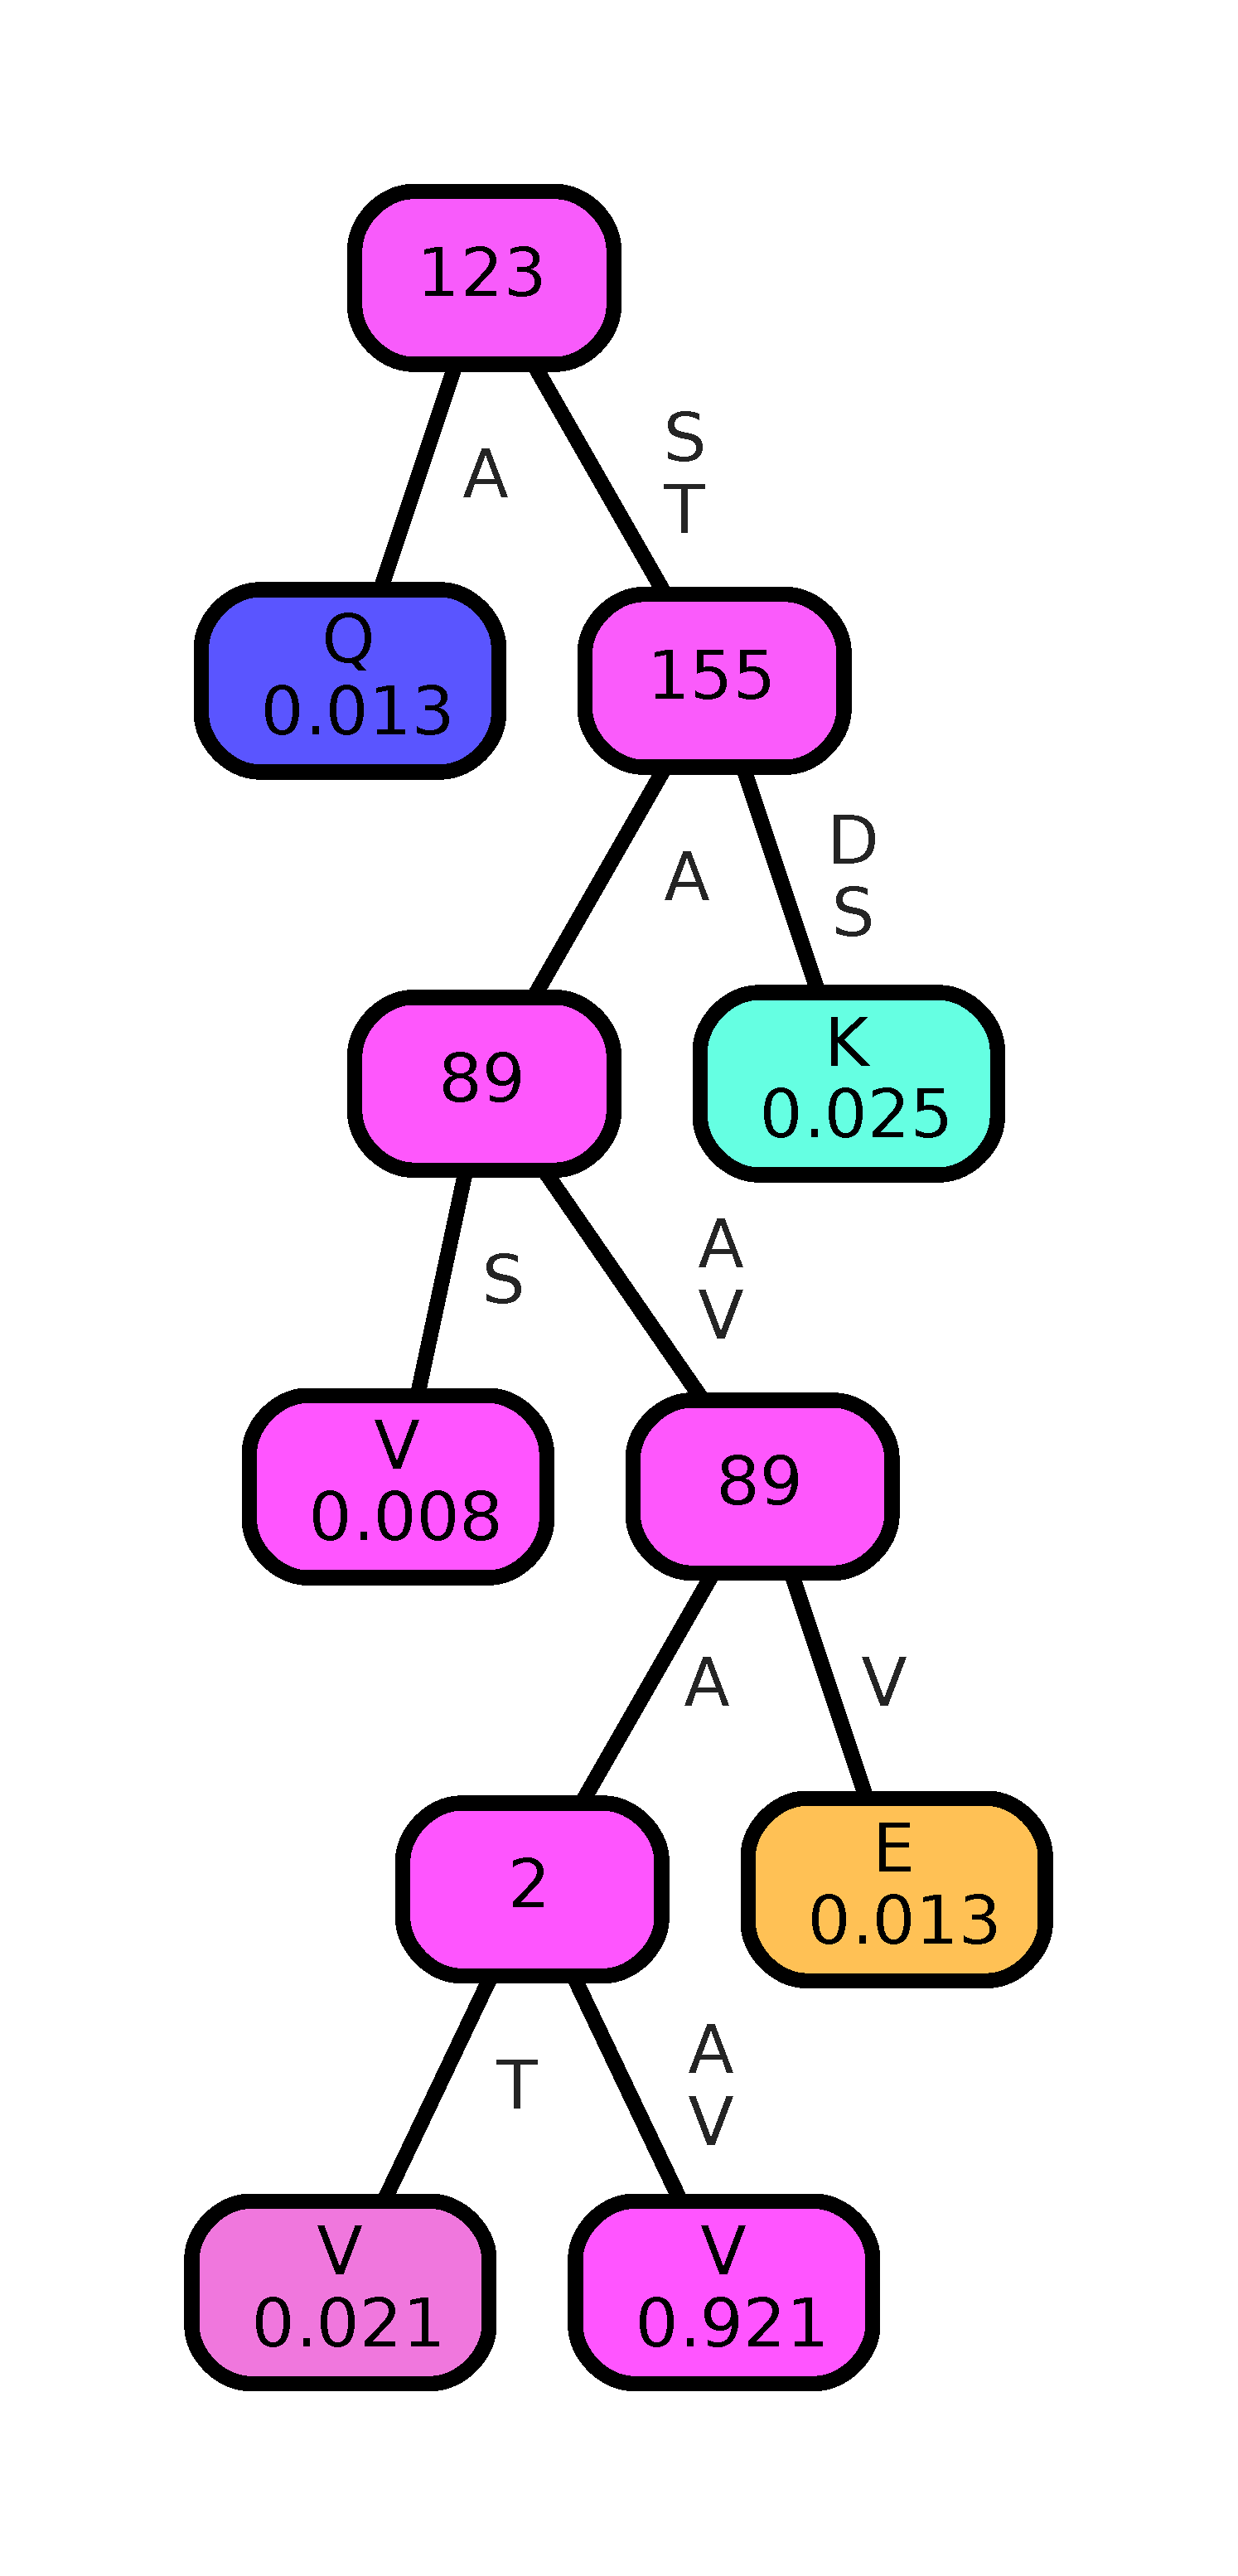
\includegraphics[width=\WDTB]{../qnet_predictions/qnet_models/trees/proc63}}; 

      
      \node[anchor=north,xcirc,inner sep=-20pt,label={[xshift=-.6in,yshift=.7in,align=center,\LCOL]-90:index\\155}] (P155) at (Z) {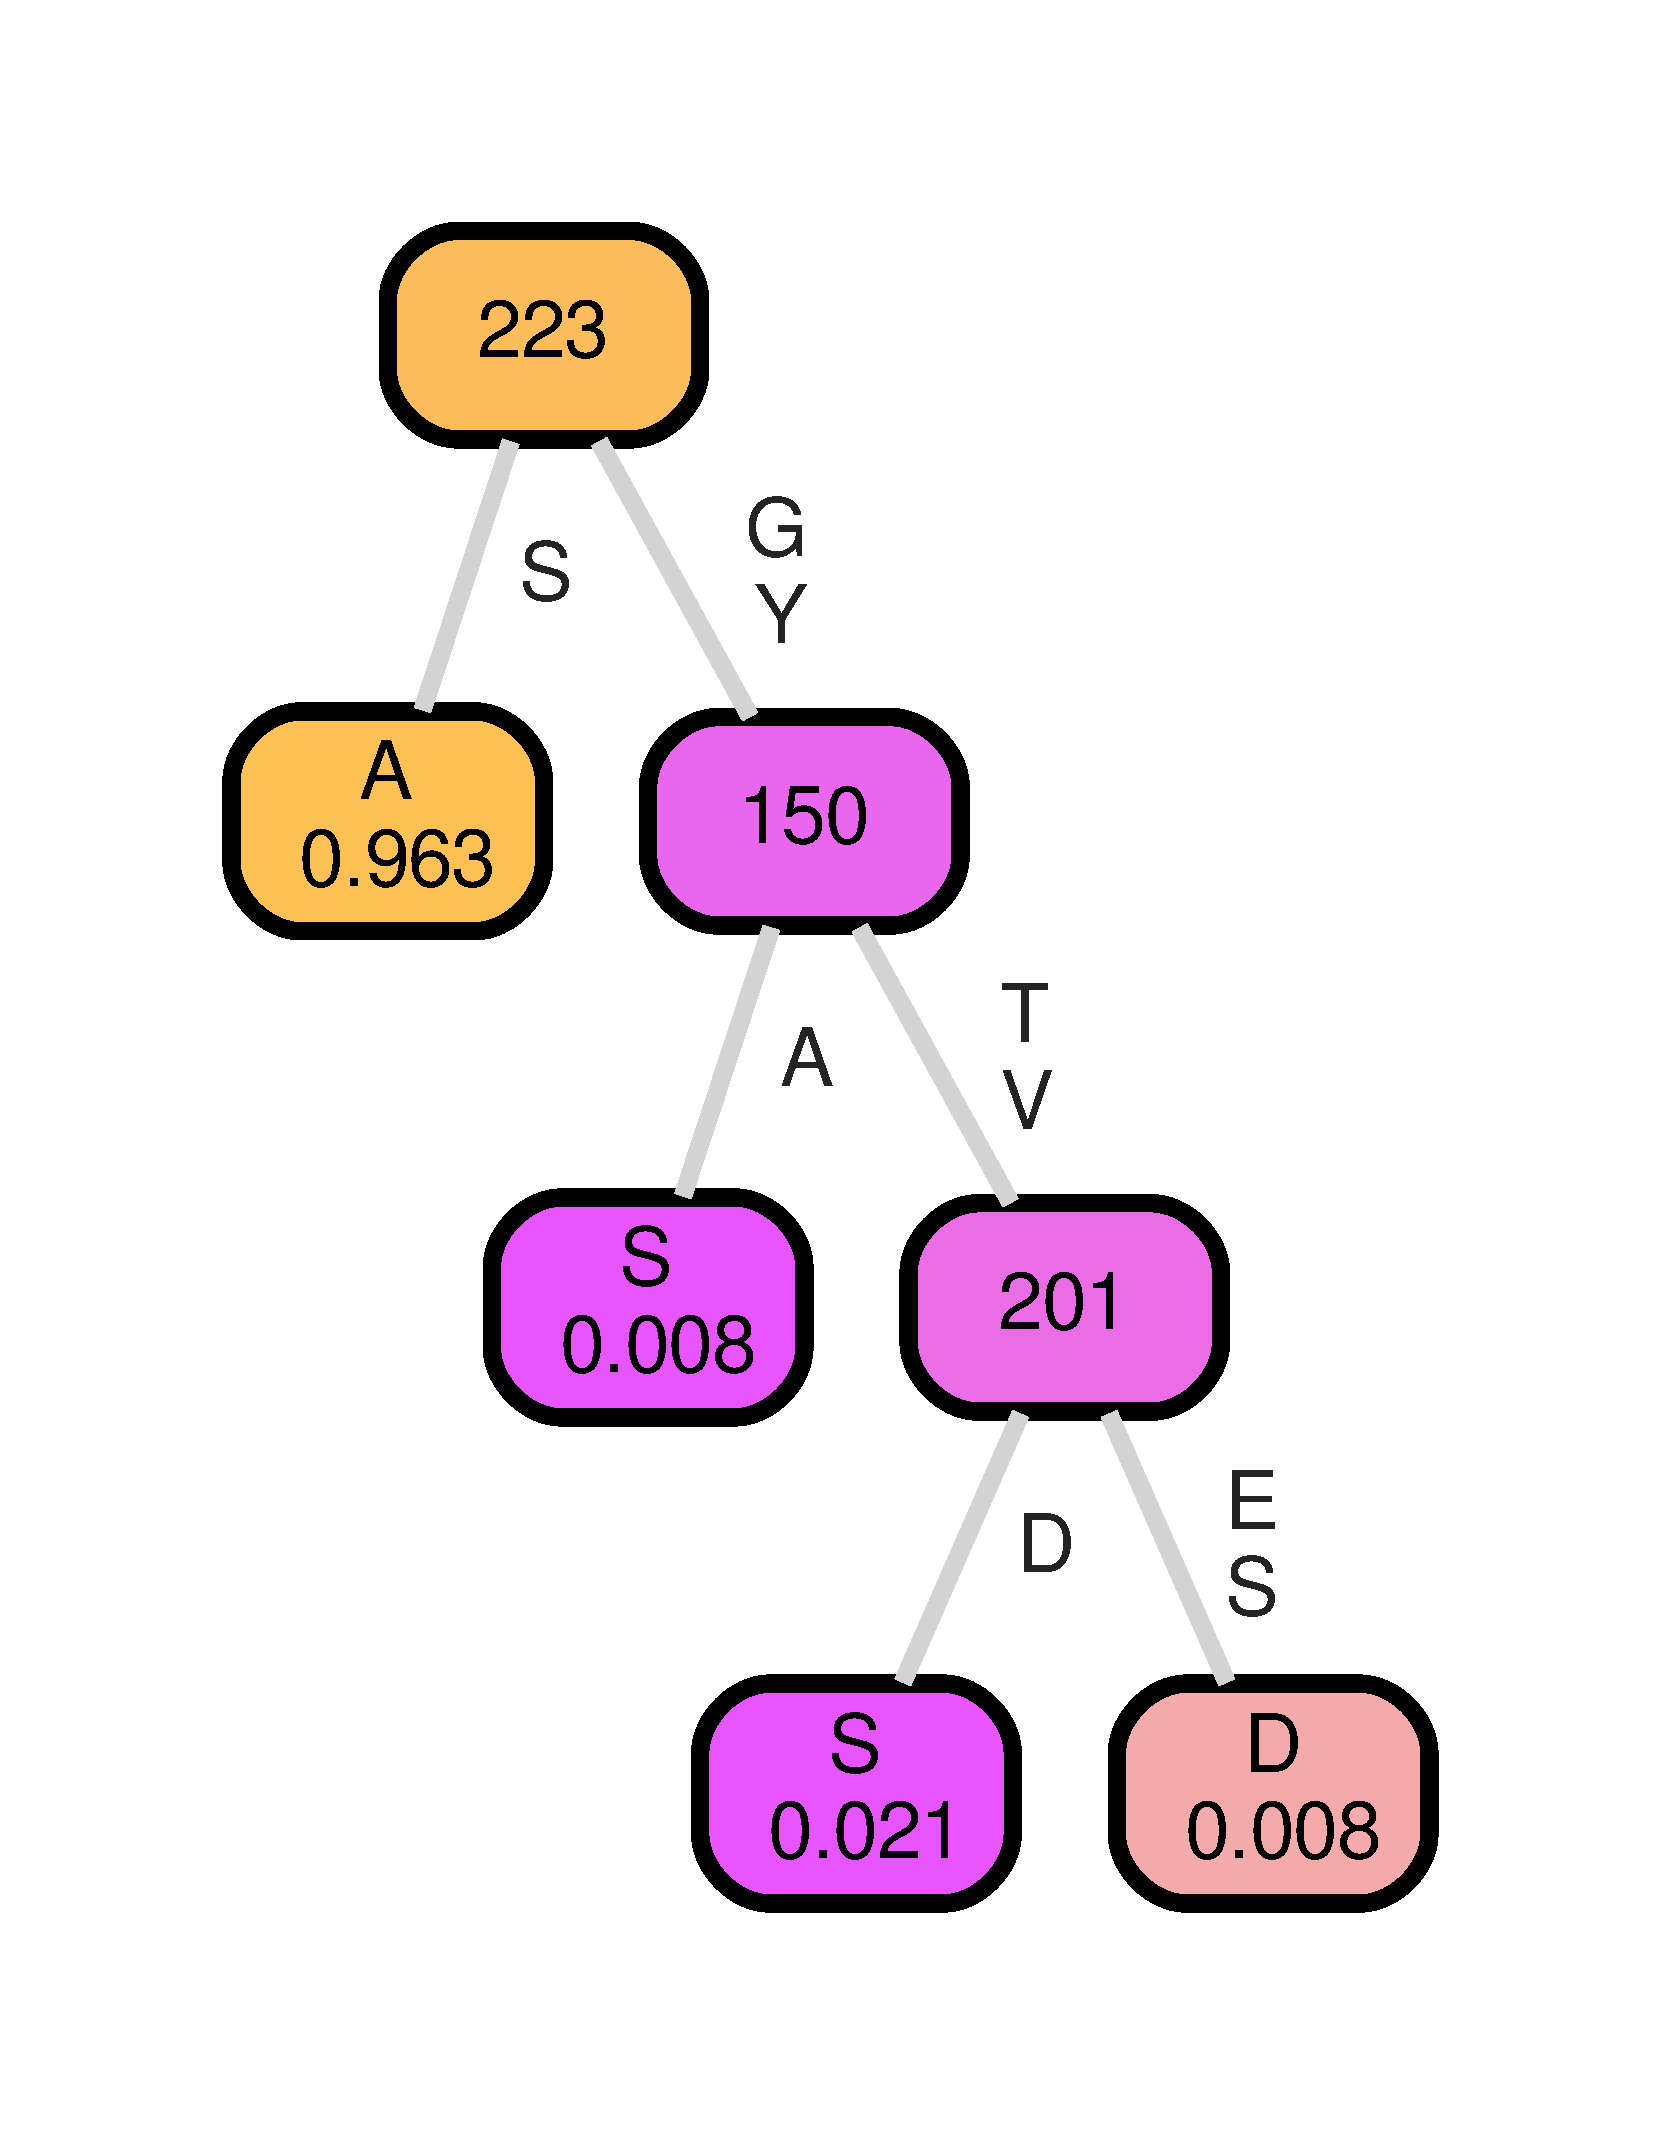
\includegraphics[width=\WDTC]{../qnet_predictions/qnet_models/trees/proc155}};

      \node[anchor=north,xcirc,inner sep=-25pt,label={[yshift=.65in,xshift=-.45in,align=center,\LCOL]-90:index\\14}] (P14) at ([xshift=-2.2in,yshift=-0.8in]P155.south) {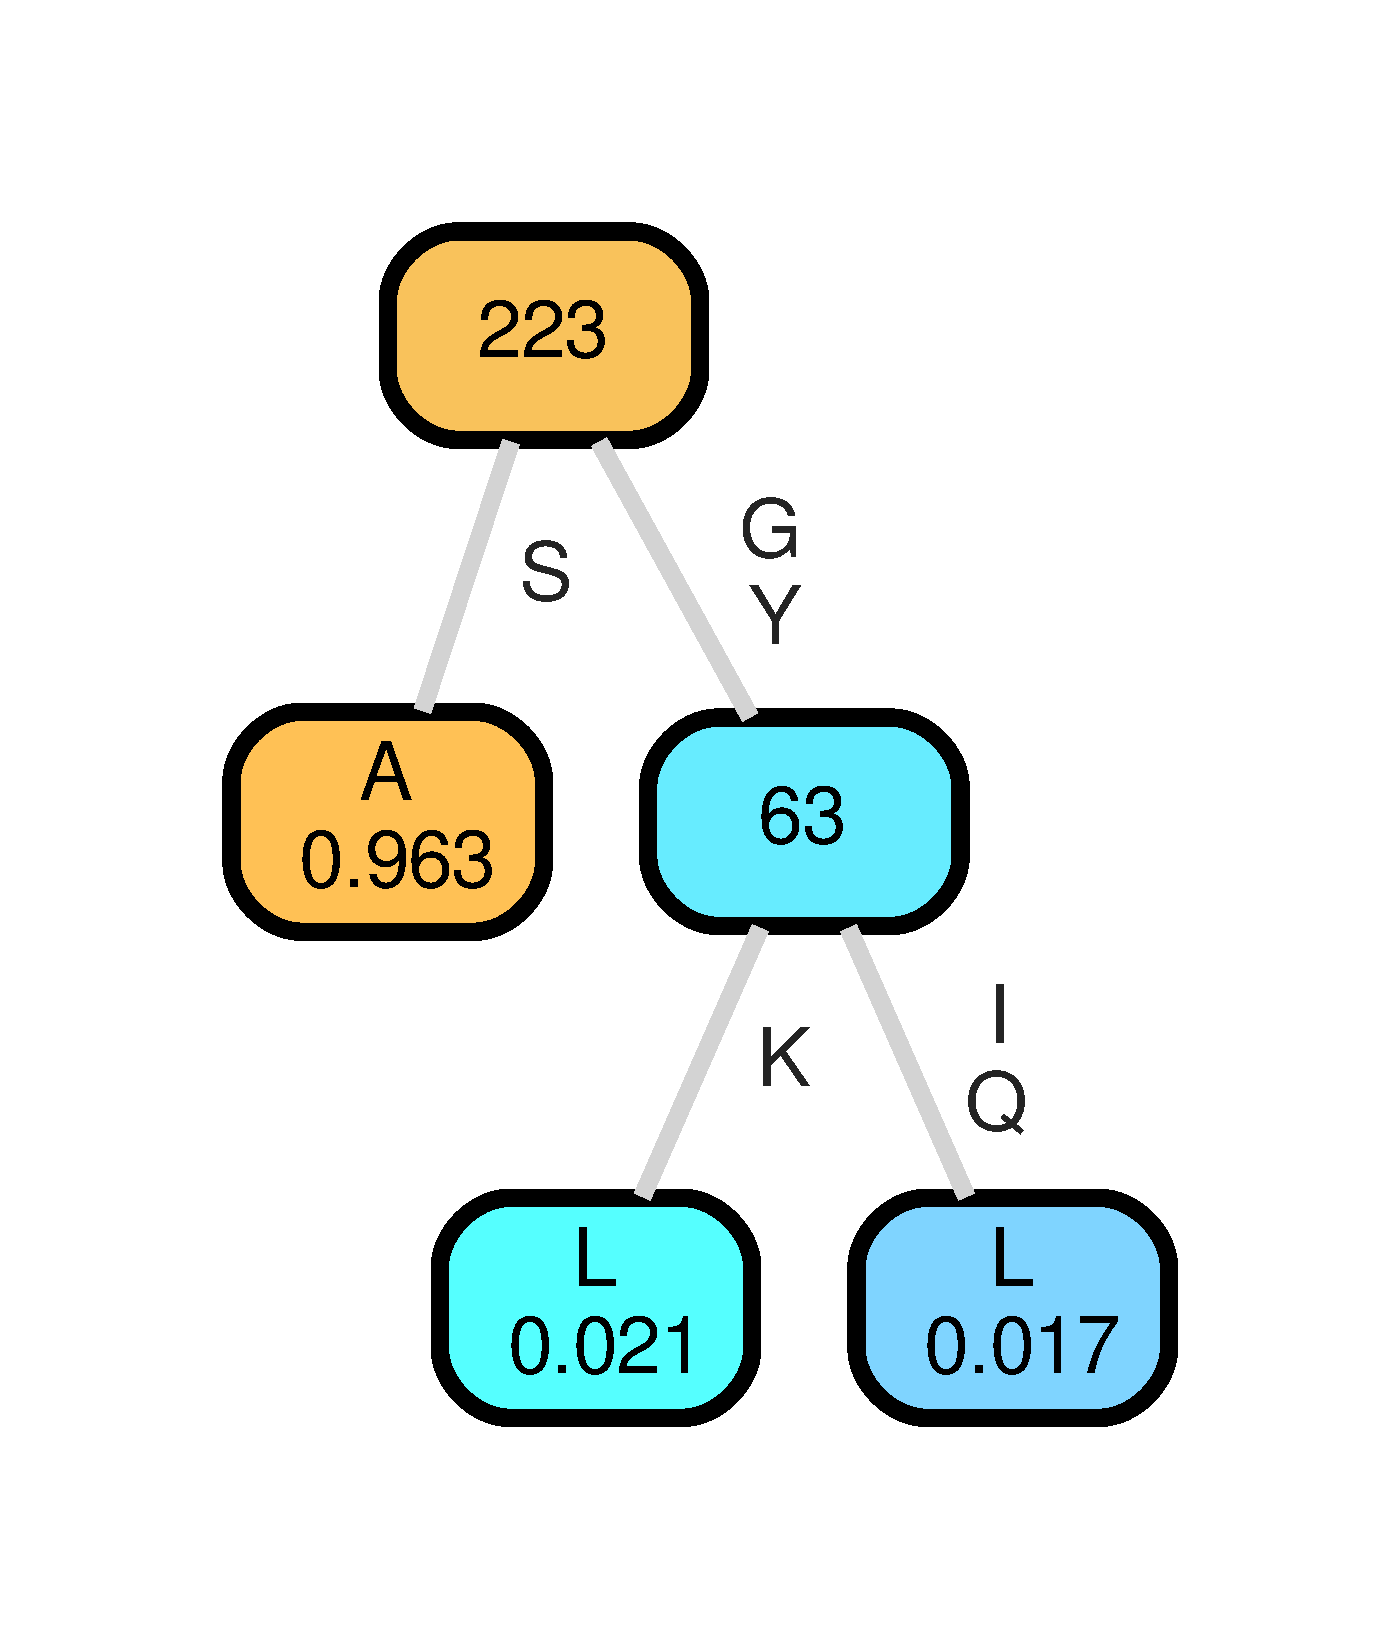
\includegraphics[width=\WDTB]{../qnet_predictions/qnet_models/trees/proc14}}; 
      
      \node[anchor=north,xcirc,inner sep=-25pt,label={[yshift=.6in,xshift=-.5in,align=center,\LCOL]-90:index\\223}] (P223) at ([xshift=-0in,yshift=-0.10in]P155.south) {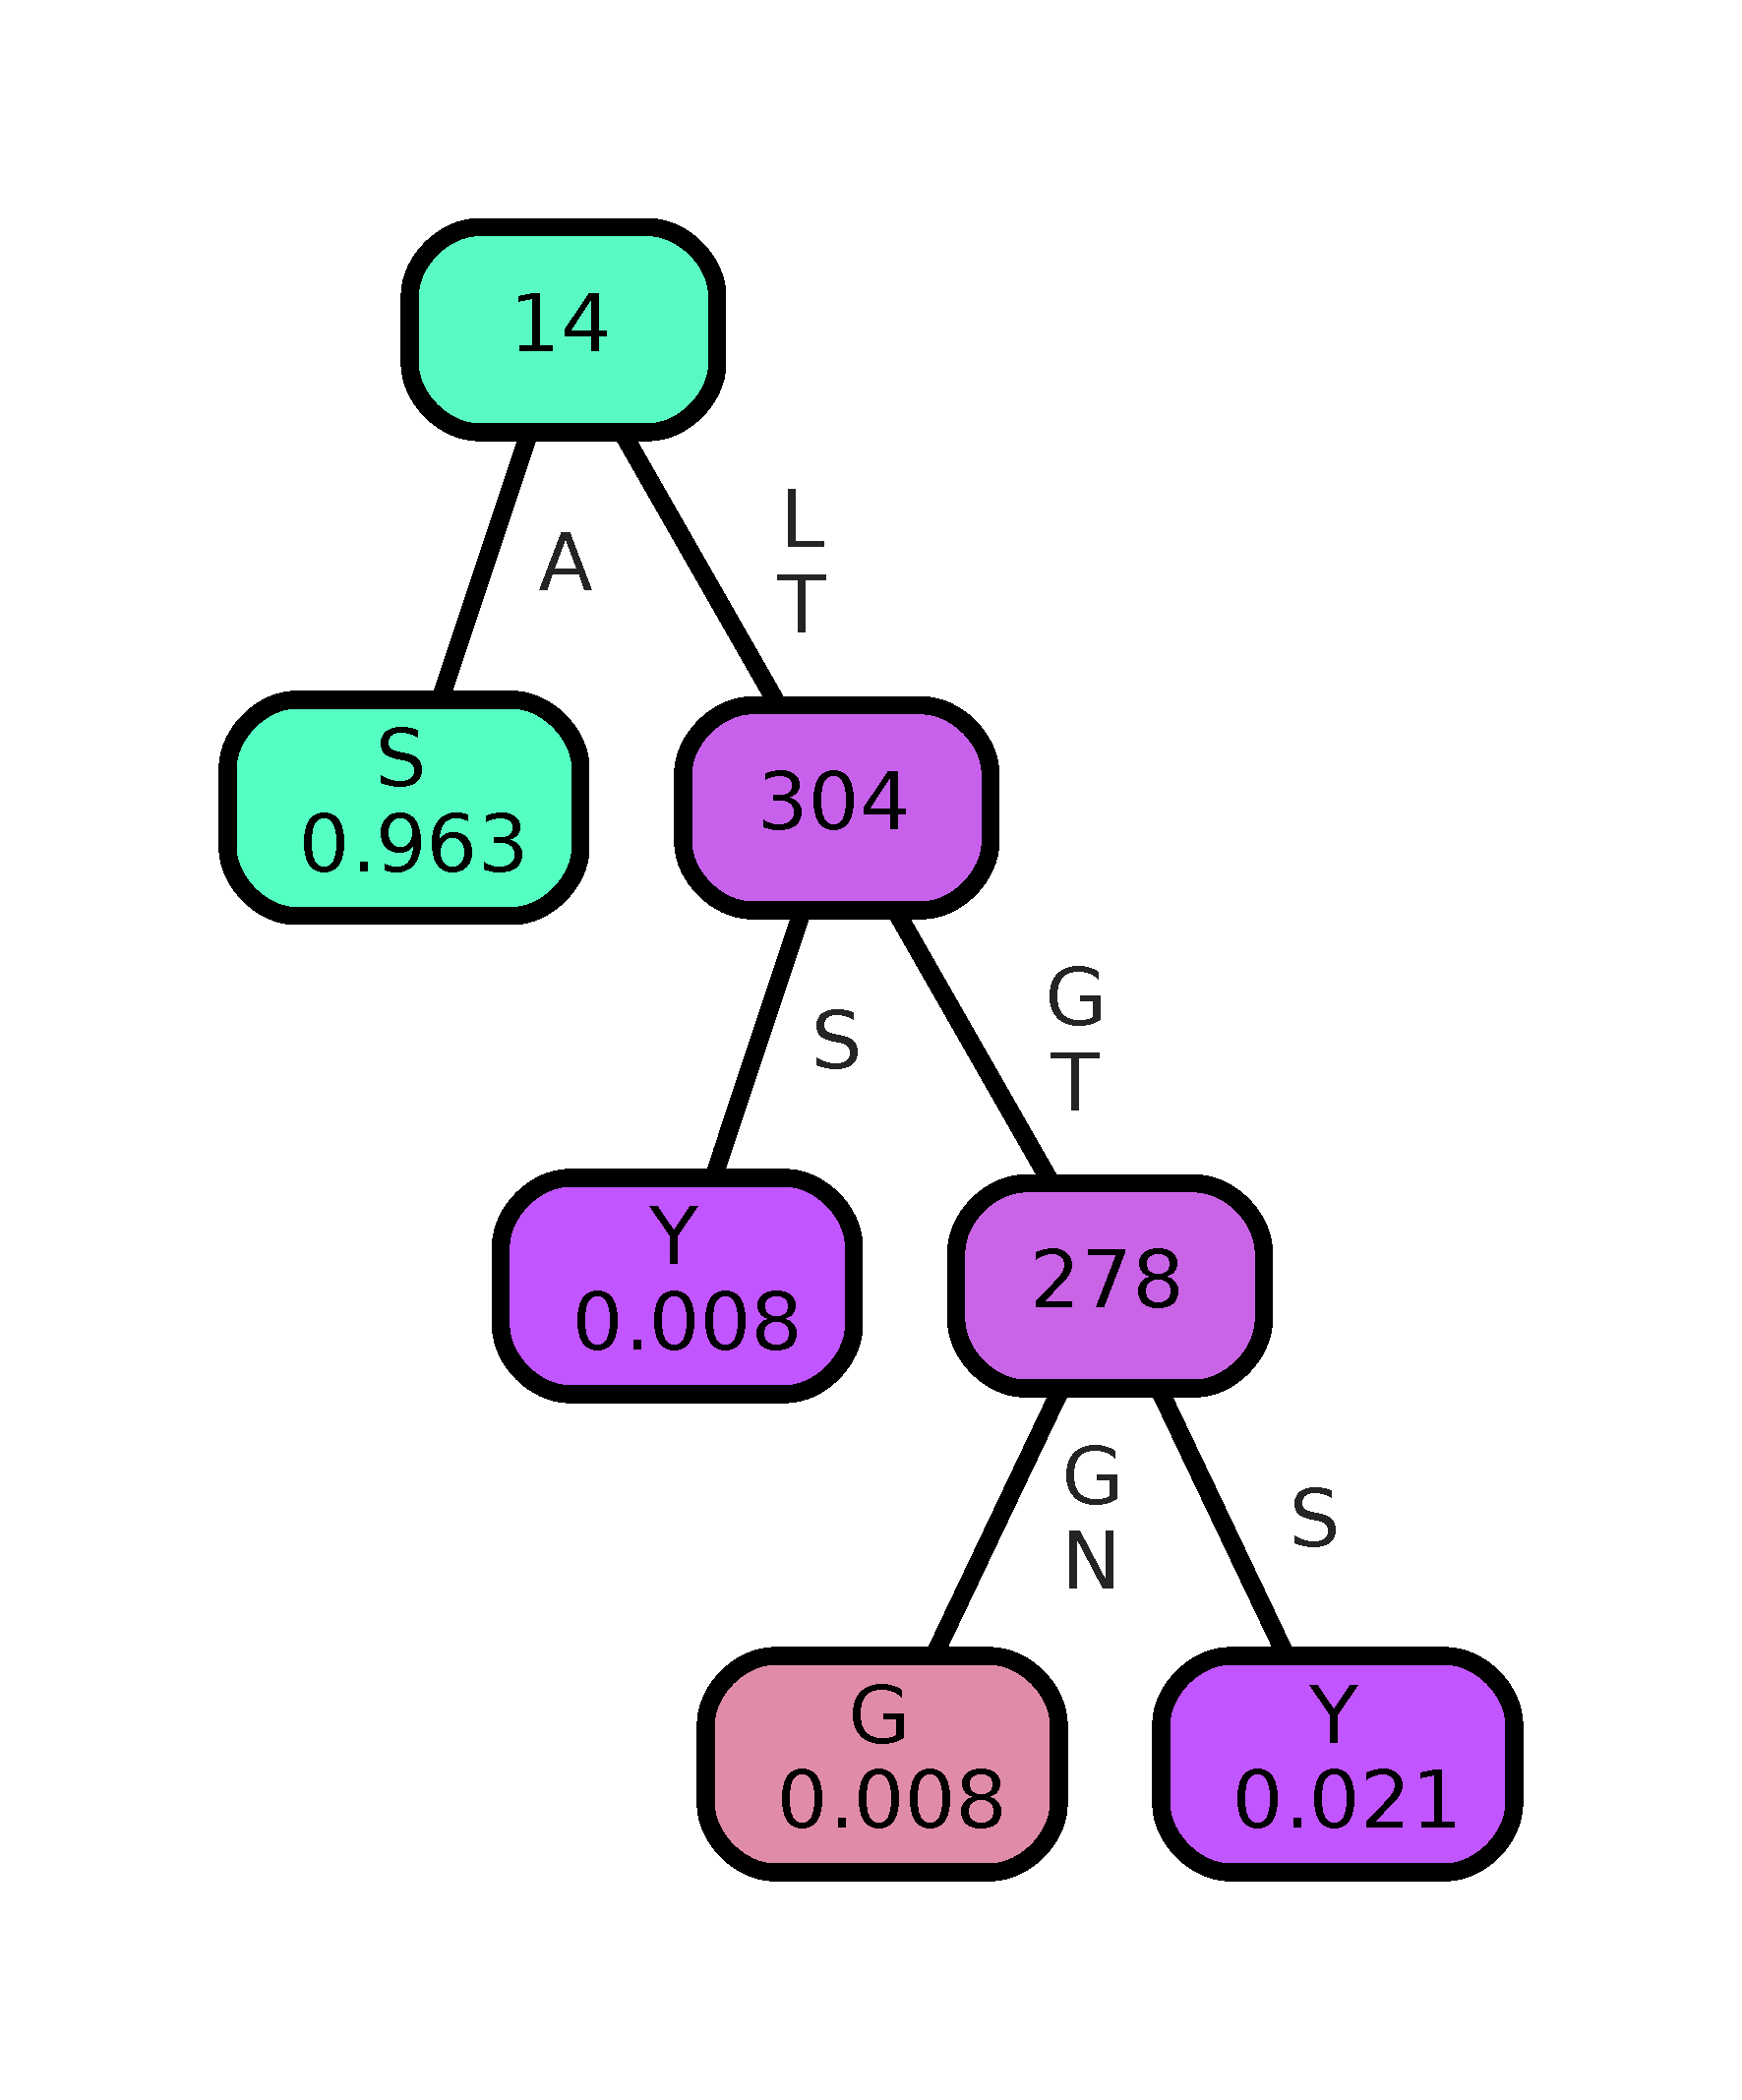
\includegraphics[width=\WDT]{../qnet_predictions/qnet_models/trees/proc223}};


      \node[text width=.13in,  rounded corners=8pt, line width=2pt,,inner sep=10pt,opacity=1,draw=\DCOLx] (X1) at ([yshift=.835in,xshift=.12in]P63) {};
      \draw [line width=\LWT,\DCOLx,-latex,] (X1)  to [out=75,in=140,looseness=1.55]  (P155);

      \node[text width=.13in,  rounded corners=8pt, line width=2pt,inner sep=10pt,opacity=1,draw=\DCOLx] (X2) at ([yshift=.845in,xshift=-.335in]P155) {};
      \draw [line width=\LWT,\DCOLx,-latex,] (X2)  to [out=0,in=60,looseness=1]  (P223);

      \node[text width=.13in,  rounded corners=8pt, line width=2pt,,inner sep=10pt,opacity=1,draw=\DCOLx] (X3) at ([yshift=.0in,xshift=.12in]P14) {};
      \draw [line width=\LWT,\DCOLx,-latex,] (X3)  to [out=150,in=-120,looseness=1.1]  (P63);

      \node[text width=.15in,  rounded corners=8pt, line width=2pt,inner sep=10pt,opacity=1,draw=\DCOLx] (X4) at ([yshift=.88in,xshift=-.34in]P223) {};
      \draw [line width=\LWT,\DCOLx,-latex,] (X4)  to [out=210,in=35,looseness=1.2]  (P14);

      \node[anchor=north,align=left,font=\bf\tt\footnotesize] (N3) at ([yshift=-6.1in,xshift=-1.85in]Z.south) {\bf\sffamily\fontsize{7}{8}\selectfont H1N1 2020-2021\\\bf\sffamily\fontsize{7}{8}\selectfont Haemagglutinin Sequences\\$\cdots$GTSRY{\color{Red1}S}KKFKPEIATRPKVRDQEGR$\cdots$\\$\cdots$GTSKY{\color{Red1}G}KKFMPEIARRPKVRNQEGR$\cdots$\\
        $\cdots$GSSKY{\color{Red1}Y}KRFTPEIVARPKVREQAGR$\cdots$\\
 $\cdots$GSSKY{\color{Red1}Y}KRFTPEIVARPKVREQAGR$\cdots$};

%A/Niger/8327/2020 
%
%A/Parana/10835/2021
%A/Gansu-Xifeng/1143/2021
%A/Sichuan/01208/2021

   \node[anchor=west,align=left,font=\bf\sffamily\fontsize{8}{10}\selectfont] (N4) at ([xshift=0.1in,yshift=.05in]N3.east) {A/Niger/8327/2020 \\
    A/Parana/10835/2021\\
      A/Gansu-Xifeng/1143/2021\\  
      A/Sichuan/01208/2021};

       \draw [ultra thick] ([yshift=.25in,xshift=.01in]N4.west) --++ (-.13in,-.190in);
       \draw [ultra thick] ([yshift=.1in,xshift=.01in]N4.west) --++ (-.13in,-.2in);
       \draw [ultra thick] ([yshift=-0.05in,xshift=.01in]N4.west) --++ (-.13in,-.2in);
       \draw [ultra thick] ([yshift=-.2in,xshift=.01in]N4.west) --++ (-.13in,-.2in);

       \node [align=center,text=IndianRed2,anchor=north] at ([xshift=-2.25in,yshift=-.1in]N4.south) {index 223};

      \node[anchor=west,rounded corners=3pt,align=center] (I1) at ([yshift=-.6in,xshift=.3in]P14.south west) {Color key (mixed colors represent distributions)};


      \definecolor{Acol}{RGB}{255,193,85}
      \definecolor{Dcol}{RGB}{255,255,85}
      \definecolor{Ecol}{RGB}{255,255,85}
      \definecolor{Gcol}{RGB}{136,255,85}
      \definecolor{Icol}{RGB}{85,255,150}
      \definecolor{Kcol}{RGB}{85,255,255}
      \definecolor{Lcol}{RGB}{85,255,255}
      \definecolor{Qcol}{RGB}{111,85,255}
      \definecolor{Scol}{RGB}{231,85,255}
      \definecolor{Tcol}{RGB}{255,85,255}
      \definecolor{Vcol}{RGB}{255,85,255}
      \definecolor{Ycol}{RGB}{255,85,97}
      
      \node[font=\bf\sffamily,anchor=north,rounded corners=3pt,text width=.1in,text height=.1in,fill=Acol,align=center,opacity=\OPC] (I1) at ([yshift=-.05in]I1.south west) {A};
      \node[font=\bf\sffamily,anchor=west,rounded corners=3pt,text width=.1in,text height=.1in,fill=Dcol,align=center,opacity=\OPC] (I1) at ([xshift=.05in]I1.east) {D};
      \node[font=\bf\sffamily,anchor=west,rounded corners=3pt,text width=.1in,text height=.1in,fill=Ecol,align=center,opacity=\OPC] (I1) at ([xshift=.05in]I1.east) {E};
      \node[font=\bf\sffamily,anchor=west,rounded corners=3pt,text width=.1in,text height=.1in,fill=Gcol,align=center,opacity=\OPC] (I1) at ([xshift=.05in]I1.east) {G};
      \node[font=\bf\sffamily,anchor=west,rounded corners=3pt,text width=.1in,text height=.1in,fill=Icol,align=center,opacity=\OPC] (I1) at ([xshift=.05in]I1.east) {I};
      \node[font=\bf\sffamily,anchor=west,rounded corners=3pt,text width=.1in,text height=.1in,fill=Kcol,align=center,opacity=\OPC] (I1) at ([xshift=.05in]I1.east) {K};
      \node[font=\bf\sffamily,anchor=west,rounded corners=3pt,text width=.1in,text height=.1in,fill=Lcol,align=center,opacity=\OPC] (I1) at ([xshift=.05in]I1.east) {L};
      \node[font=\bf\sffamily,anchor=west,rounded corners=3pt,text width=.1in,text height=.1in,fill=Qcol,align=center,opacity=\OPC] (I1) at ([xshift=.05in]I1.east) {Q};
      \node[font=\bf\sffamily,anchor=west,rounded corners=3pt,text width=.1in,text height=.1in,fill=Scol,align=center,opacity=\OPC] (I1) at ([xshift=.05in]I1.east) {S};
      \node[font=\bf\sffamily,anchor=west,rounded corners=3pt,text width=.1in,text height=.1in,fill=Tcol,align=center,opacity=\OPC] (I1) at ([xshift=.05in]I1.east) {T};
      \node[font=\bf\sffamily,anchor=west,rounded corners=3pt,text width=.1in,text height=.1in,fill=Vcol,align=center,opacity=\OPC] (I1) at ([xshift=.05in]I1.east) {V};
      \node[font=\bf\sffamily,anchor=west,rounded corners=3pt,text width=.1in,text height=.1in,fill=Ycol,align=center,opacity=\OPC] (I1) at ([xshift=.05in]I1.east) {Y};

      % \node[font=\bf\sffamily,anchor=north,rounded corners=3pt,text width=.1in,text height=.1in,fill=DarkOrange3!70,align=center,opacity=\OPC] (I1) at ([yshift=-.05in]I1.south) {A};

      % \node[font=\bf\sffamily,anchor=north,rounded corners=3pt,text width=.1in,text height=.1in,fill=SeaGreen2,align=center,opacity=\OPC] (I1) at ([yshift=-.05in]I1.south) {C};

      % \node[font=\bf\sffamily,anchor=north,rounded corners=3pt,text width=.1in,text height=.1in,fill=DodgerBlue2!80,align=center,opacity=\OPC] (I1) at ([yshift=-.050in]I1.south) {G};
    \end{tikzpicture}
  };

  \node [anchor=south west] (L1) at ([yshift=-.2650in]T.north west) {\Large a.};
  \node [anchor=south west] (L2) at ([yshift=-3.25in]T.north west) {\Large c.};
  \node [anchor=south west] (L3) at ([yshift=-5.65in]T.north west) {\Large d.};

\end{tikzpicture}

 \else
  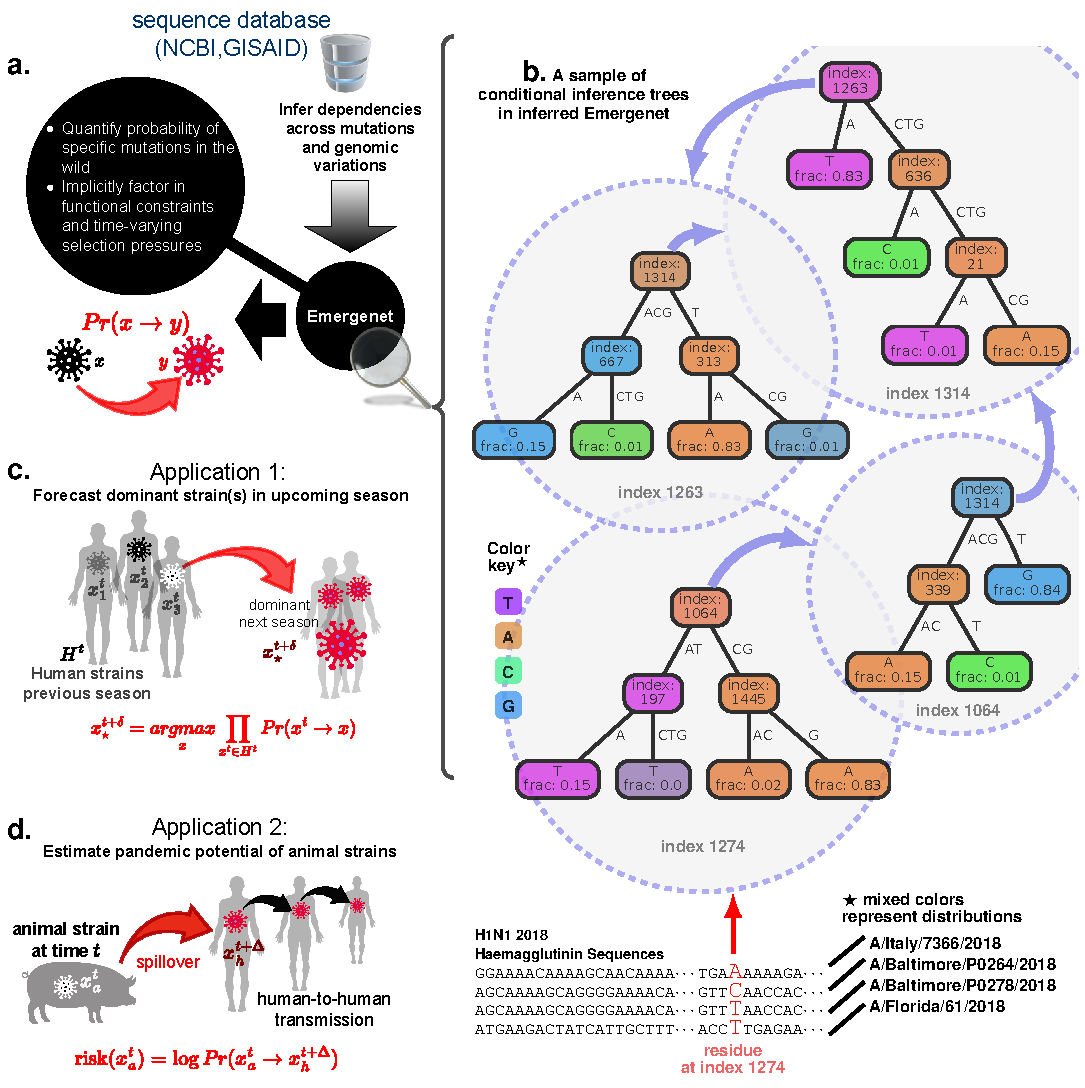
\includegraphics[width=\textwidth]{Figures/External/scheme}
  \fi
  \vspace{-20pt}
  
 \captionN{\textbf{\enet inference and applications}. \textbf{a}, Variations of
   genomes for identical subgroups of \infl are analyzed to infer a recursive forest of conditional inference trees~\cite{Hothorn06unbiasedrecursive} -- the \enet --   which maximally captures the emergent  dependencies between an a priori unspecified number of   mutations, deletions and insertions. With these inferred dependencies we can    estimate the numerical odds of specific mutations, and by extension, the numerical value of
   the probability of one strain giving rise to another in the wild, under  complex selection pressures from the background. b, Snapshot of decision trees  from the
   \enet constructed for H1N1 haemagglutinnin 2018 sequences. Note that the decision tree predicting the bases at index 1274   uses the bases at 1064, 1445, 197 as features. These features are automatically selected, as being maximally predictive  of the bases be at 1274. Then, we compute predictors for each of these  feature indices, $e.g.$   trees for  index 1064, which involves index 1314 and 339 as features. Continuing, we find that the trees for index 1314 involves indices 1263, 636 and 21, and that for 1263 involves 1314, 667 and 313. The predictor for 1263  depends on 1314, and that for 1314 depends on 1263, revealing the recursive structure of \enet. c, First application: With \enet induced ability to quantify mutation probabilities,  we forecast  dominant strain(s) for the next flu season, using only  sequences collected in the previous season (and the inferred \enet, using data from the past year). d, Second application: estimation of the risk of a global pandemic posed by individual animal strains that are still not known to circulate in humans.}\label{figscheme}.
\end{figure*}
\else
\refstepcounter{figure}\label{figscheme}
\fi  
%#############################################                                  
%#############################################                                  
%#############################################
%#############################################
\ifFIGS
\begin{figure*}[!ht]
  \centering
  \tikzexternalenable
   \tikzsetnextfilename{seasonalpred_both}

  \tikzXtrue 
  \iftikzX
  \hspace{-20pt}\resizebox{.975\linewidth}{!}{\begin{tikzpicture}
  \def\HGT{.35in}
  \def\WDT{2.75in}
  \def\YST{-.3in}

  \node[,label={[font=\bf\sffamily,yshift=-.60in]90:\underline{Southern Hemisphere (Prediction in December)}}] (AAA) at (0,0) {\pgfplotsset{
  discard if/.style 2 args={
    x filter/.append code={
      \edef\tempa{\thisrow{#1}}
      \edef\tempb{#2}
      \ifx\tempa\tempb
      \def\pgfmathresult{inf}
      \fi
    }
  },
  discard if not/.style 2 args={
    x filter/.append code={
      \edef\tempa{\thisrow{#1}}
      \edef\tempb{#2}
      \ifx\tempa\tempb
      \else
      \def\pgfmathresult{inf}
      \fi
    }
  }
}

\begin{tikzpicture}

  \def\NNX{1}
  \noexpand\def\YMAX{15}
  \def\YLABEL{}
  \newcommand{\PPX}[3][2001]{
    \begin{axis}[name=XX,\TEXTCOL,anchor=center,
      title={},legend columns=1,
      legend style={text=black,anchor=west,at={(0.5,1.8)},
        inner sep=1pt,draw=none,fill=black!5,fill opacity=.75,align=right,
        text opacity=1,/tikz/column 2/.style={
          column sep=5pt,
        },},
      ymax=0,
      ymin=-\YMAX,
      xmin=#1,
      xmax=2022,
      name=X0,
      anchor=center,
      width=\WDT,
      height=\HGT,
      scale only axis=true,
      enlargelimits=false,
      enlarge y limits=false,
      enlarge x limits=0.06,
      axis on top=false,
      axis line style={black!2, very thick},
      grid=both,minor x tick num=3,
      major grid style={opacity=1,,thick,black!10},
      minor grid style={opacity=1,,semithick,Red4!5},
      major tick length=0pt,
      minor tick length=0pt,
      ytick style={draw=none},
      scaled y ticks = false,
      y tick label style={/pgf/number format/fixed,
        /pgf/number format/1000 sep = \empty % \thinspace optional
      },
      x tick label style={/pgf/number format/fixed,
        /pgf/number format/1000 sep = \empty % Optional
      },
      xlabel={year},ylabel style={yshift=1in,align=center,xshift=1.9in},
      xlabel style={yshift=.05in},ybar,,bar width=\BWIDTH,
      ytick={#2},xtick={2000,2004,2008,2012,2016,2020},xticklabels={},xlabel={},ylabel={\YLABEL},,ylabel style={yshift=-.8in,align=center,xshift=-1.9in},
      xtick=data, xticklabel style={rotate=90}]
      
      \addplot [area legend,restrict x to domain=0:2022,negstyle]
      table [col sep=comma,x expr=\coordindex+#1,
      y expr=(\thisrow{\NMX}
      -\thisrow{ldistance_WHO})/(\NNX)] {\DATAQNETx};
    \end{axis}
    % 
    \begin{axis}[\TEXTCOL,anchor=center,yshift=\HGT,
      title={},legend columns=1,legend style={text=black,anchor=west,at={(0.5,.8)},
        inner sep=1pt,draw=none,fill=black!5,fill opacity=.75,align=right,
        text opacity=1,/tikz/column 2/.style={
          column sep=5pt,
        },},
      ymin=0,
      ymax=\YMAX,
      xmax=2022,
      xmin=#1,
      name=X0,
      anchor=center,
      width=\WDT,
      height=\HGT,
      scale only axis=true,
      enlargelimits=false,
      enlarge y limits=false,
      enlarge x limits=0.06,
      axis on top=false,
      axis line style={black!2, very thick},
      grid=both,minor x tick num=3,
      major grid style={opacity=1,,thick,black!10},
      minor grid style={opacity=1,,semithick,Red4!5},
      major tick length=0pt,
      minor tick length=0pt,
      ytick style={draw=none},
      scaled y ticks = false,
      y tick label style={/pgf/number format/fixed,
        /pgf/number format/1000 sep = \empty % \thinspace optional
      },
      x tick label style={/pgf/number format/fixed,
        /pgf/number format/1000 sep = \empty % Optional
      },
      xlabel={year},ylabel style={yshift=0.8in,align=center,xshift=1in},
      xlabel style={yshift=.05in},ybar,,bar width=\BWIDTH,ytick={#3},,xtick={2000,2004,2008,2012,2016,2020},xticklabels={},xlabel={},
      xtick=data, xticklabel style={rotate=90}]
      
      \addplot [area legend,restrict x to domain=0:2022,posstyle]
      table [col sep=comma,x expr=\coordindex+#1,y expr=(\thisrow{\NMX}-\thisrow{ldistance_WHO})/(\NNX)] {\DATAQNETx};
    \end{axis}

    \begin{axis}[\TEXTCOL,anchor=center,yshift=0,
      title={},legend columns=1,legend style={text=black,anchor=west,at={(0.5,.8)},
        inner sep=1pt,draw=none,fill=black!5,fill opacity=.75,align=right,
        text opacity=1,/tikz/column 2/.style={
          column sep=5pt,
        },},
      ymin=0,
      ymax=\YMAX,
      xmax=2022, 
      xmin=#1,
      name=X0,
      anchor=center,
      width=\WDT,
      height=\HGT,
      scale only axis=true,
      enlargelimits=false,
      enlarge y limits=false,
      enlarge x limits=0.060,
      axis on top=false,
      axis line style={black!2, very thick},
      % grid,
      grid style={opacity=1,dashed,thick,black!10},
      major tick length=0pt,
      ytick style={draw=none},
      scaled y ticks = false,
      y tick label style={/pgf/number format/fixed,
        /pgf/number format/1000 sep = \empty % \thinspace optional
      },
      x tick label style={/pgf/number format/fixed,
        /pgf/number format/1000 sep = \empty % Optional
      },
      xlabel={year},ylabel style={yshift=0.2in,align=center,xshift=1in},
      xlabel style={yshift=.05in},ybar,
      ,bar width=\BWIDTH,ytick={},yticklabels={},
      ,xtick={2000,2004,2008,2012,2016,2020},xlabel={},
      xtick=data, xticklabel style={rotate=90}]
      
      \addplot [area legend,restrict x to domain=0:2022,draw=none,fill=none]
      table [col sep=comma,x expr=\coordindex+#1,y expr=0] {\DATAQNETx};
    \end{axis}
  }

  \def\TEXTCOL{gray}
  \def\RCLR{IndianRed1}
  \def\RCLRB{IndianRed1}
  \def\QCLRC{Orchid3}
  \def\QCLD{gray!50}
  \def\QCLRB{black}
  \def\QCLR{black}
  \def\YST{-.3in}
  \noexpand\def\PCOL{black!0}
  \noexpand\def\NCOL{black!0}
  \noexpand\def\PCOLf{black!90}
  \noexpand\def\NCOLf{Red1}
  \def\SC{1.35}
  \def\XCOL{lightgray!70}
  \def\BWIDTH{8.2pt}
  \tikzset{%
    posstyle/.style =   {line width=1pt,
      draw=\PCOL,fill=\PCOLf}}
  \tikzset{%
    negstyle/.style =   {line width=1pt,
      draw=\NCOL,fill=\NCOLf}}
  \def\HGT{.3in}
  \def\WDT{2.75in}

  \def\YTICKA{0,-5,-10}
  \def\YTICKB{0,5,10}
\def\NMX{ldistance_Qnet_recommendation}
  \node[anchor=north west] (A) at (0,0) {\begin{tikzpicture}[anchor=center,font=\bf\sffamily\fontsize{8}{9}\selectfont]
      \def\DATAQNETx{Figures/plotdata/south_h1n1_ha.csv}
      \def\YLABEL{}
      \PPX[2001]{\YTICKA}{\YTICKB}
    \end{tikzpicture}};

  \node[anchor=north west] (B) at ([yshift=\YST]A.south west) {\begin{tikzpicture}[anchor=center,font=\bf\sffamily\fontsize{8}{9}\selectfont]
      \def\DATAQNETx{Figures/plotdata/south_h1n1_na.csv}
      \def\YLABEL{}
      \PPX[2001]{\YTICKA}{\YTICKB}
    \end{tikzpicture}};

  \node[anchor=north west] (C) at ([xshift=-.25in,yshift=0in]A.north east) {\begin{tikzpicture}[anchor=center,font=\bf\sffamily\fontsize{8}{9}\selectfont]
      \def\DATAQNETx{Figures/plotdata/south_h3n2_ha.csv}
      \def\YLABEL{}
      \PPX[2005]{\YTICKA}{\YTICKB}
    \end{tikzpicture}};

  \node[anchor=north west] (D) at ($(B.north west)!(C.west)!(B.north east)$) {\begin{tikzpicture}[anchor=center,font=\bf\sffamily\fontsize{8}{9}\selectfont]
      \def\DATAQNETx{Figures/plotdata/south_h3n2_na.csv}
      \def\YLABEL{}
      \PPX[2003]{\YTICKA}{\YTICKB}
    \end{tikzpicture}};

\def\NMX{ldistance_Qnet_recommendation_0}

  \node[anchor=north west] (E) at ([yshift=\YST]B.south west) {\begin{tikzpicture}[anchor=center,font=\bf\sffamily\fontsize{8}{9}\selectfont]
      \def\DATAQNETx{Figures/plotdata/south_h1n1_na_3cluster.csv}
      \def\YLABEL{}
      \PPX[2001]{\YTICKA}{\YTICKB}
    \end{tikzpicture}};



  \node[anchor=north west] (F) at ($(E.north west)!(D.west)!(E.north east)$) {\begin{tikzpicture}[anchor=center,font=\bf\sffamily\fontsize{8}{9}\selectfont]
      \def\DATAQNETx{Figures/plotdata/south_h3n2_na_3cluster.csv}
      \def\YLABEL{}
      \PPX[2003]{\YTICKA}{\YTICKB}
    \end{tikzpicture}};



  
  \node[anchor=south west] (L1) at ([yshift=0in,xshift=.55in]A.north west) {{\Large a.} Influenza A H1N1 HA};
  \node[anchor=south west] (L2) at ([xshift=0in]$(L1.north west)!(B.north)!(L1.south west)$) {{\Large b.} Influenza A H1N1 NA};
  \node[anchor=south west] (L3) at ([xshift=0.55in]$(L1.south west)!(C.west)!(L1.south east)$) {{\Large c.} Influenza A H3N2 HA};
  \node[anchor=south west] (L4) at ($(L2.south west)!(L3.west)!(L2.south east)$) {{\Large d.} Influenza A H3N2 NA};

  \node[anchor=south west] (L5) at ([xshift=0in]$(L2.north west)!(E.north)!(L2.south west)$) {{\Large e.} Influenza A H1N1 NA (multi-cluster)};
  \node[anchor=south west] (L4) at ($(L5.south west)!(L4.west)!(L5.south east)$) {{\Large f.} Influenza A H3N2 NA (multi-cluster)};



  
   \node[opacity=1,fill=\PCOLf,text width=.5in,text height=.05in,label={[text=\PCOLf,fill=white,font=\bf\sffamily\fontsize{9}{6}\selectfont]0:WHO better}] (X1) at ([yshift=1.2in]$(A.west)!.70!2:(C.west)$) {};
   \node[opacity=1,fill=\NCOLf,text width=.5in,text height=.05in,label={[text=\NCOLf,fill=white,font=\bf\sffamily\fontsize{9}{6}\selectfont]0:\enet better},anchor=north west] (X1) at ([xshift=1.2in]X1.north east) {};

\end{tikzpicture}
};
  \node[anchor=north,label={[font=\bf\sffamily]90:\underline{Northern Hemisphere (Prediction in February)}}] (BBB) at ([yshift=-.25in]AAA.south) {\pgfplotsset{
  discard if/.style 2 args={
    x filter/.append code={
      \edef\tempa{\thisrow{#1}}
      \edef\tempb{#2}
      \ifx\tempa\tempb
      \def\pgfmathresult{inf}
      \fi
    }
  },
  discard if not/.style 2 args={
    x filter/.append code={
      \edef\tempa{\thisrow{#1}}
      \edef\tempb{#2}
      \ifx\tempa\tempb
      \else
      \def\pgfmathresult{inf}
      \fi
    }
  }
}

\begin{tikzpicture}

  \def\NNX{1}
  \noexpand\def\YMAX{15}
  \def\YLABEL{}
  \newcommand{\PPX}[3][2001]{
    \begin{axis}[name=XX,\TEXTCOL,anchor=center,
      title={},legend columns=1,
      legend style={text=black,anchor=west,at={(0.5,1.8)},
        inner sep=1pt,draw=none,fill=black!5,fill opacity=.75,align=right,
        text opacity=1,/tikz/column 2/.style={
          column sep=5pt,
        },},
      ymax=0,
      ymin=-\YMAX,
      xmin=#1,
      xmax=2022,
      name=X0,
      anchor=center,
      width=\WDT,
      height=\HGT,
      scale only axis=true,
      enlargelimits=false,
      enlarge y limits=false,
      enlarge x limits=0.06,
      axis on top=false,
      axis line style={black!2, very thick},
      grid=both,minor x tick num=3,
      major grid style={opacity=1,,thick,black!10},
      minor grid style={opacity=1,,semithick,Red4!5},
      major tick length=0pt,
      minor tick length=0pt,
      ytick style={draw=none},
      scaled y ticks = false,
      y tick label style={/pgf/number format/fixed,
        /pgf/number format/1000 sep = \empty % \thinspace optional
      },
      x tick label style={/pgf/number format/fixed,
        /pgf/number format/1000 sep = \empty % Optional
      },
      xlabel={year},ylabel style={yshift=1in,align=center,xshift=1.9in},
      xlabel style={yshift=.05in},ybar,,bar width=\BWIDTH,
      ytick={#2},%xtick={2000,2004,2008,2012,2016,2020}
      ,xticklabels={},xlabel={},ylabel={\YLABEL},,ylabel style={yshift=-.8in,align=center,xshift=-1.9in},
      xtick=data, xticklabel style={rotate=90}]
      
      \addplot [area legend,restrict x to domain=0:2022,negstyle]
      table [col sep=comma,x expr=\coordindex+#1,
      y expr=(\thisrow{\NMX}
      -\thisrow{ldistance_WHO})/(\NNX)] {\DATAQNETx};
    \end{axis}
    % 
    \begin{axis}[\TEXTCOL,anchor=center,yshift=\HGT,
      title={},legend columns=1,legend style={text=black,anchor=west,at={(0.5,.8)},
        inner sep=1pt,draw=none,fill=black!5,fill opacity=.75,align=right,
        text opacity=1,/tikz/column 2/.style={
          column sep=5pt,
        },},
      ymin=0,
      ymax=\YMAX,
      xmax=2022,
      xmin=#1,
      name=X0,
      anchor=center,
      width=\WDT,
      height=\HGT,
      scale only axis=true,
      enlargelimits=false,
      enlarge y limits=false,
      enlarge x limits=0.06,
      axis on top=false,
      axis line style={black!2, very thick},
      grid=both,minor x tick num=3,
      major grid style={opacity=1,,thick,black!10},
      minor grid style={opacity=1,,semithick,Red4!5},
      major tick length=0pt,
      minor tick length=0pt,
      ytick style={draw=none},
      scaled y ticks = false,
      y tick label style={/pgf/number format/fixed,
        /pgf/number format/1000 sep = \empty % \thinspace optional
      },
      x tick label style={/pgf/number format/fixed,
        /pgf/number format/1000 sep = \empty % Optional
      },
      xlabel={year},ylabel style={yshift=0.8in,align=center,xshift=1in},
      xlabel style={yshift=.05in},ybar,,bar width=\BWIDTH,ytick={#3},,%xtick={2000,2004,2008,2012,2016,2020},
      xticklabels={},xlabel={},xtick=data, xticklabel style={rotate=90}]
      
      \addplot [area legend,restrict x to domain=0:2022,posstyle]
      table [col sep=comma,x expr=\coordindex+#1,y expr=(\thisrow{\NMX}-\thisrow{ldistance_WHO})/(\NNX)] {\DATAQNETx};
    \end{axis}

    \begin{axis}[\TEXTCOL,anchor=center,yshift=0,
      title={},legend columns=1,legend style={text=black,anchor=west,at={(0.5,.8)},
        inner sep=1pt,draw=none,fill=black!5,fill opacity=.75,align=right,
        text opacity=1,/tikz/column 2/.style={
          column sep=5pt,
        },},
      ymin=0,
      ymax=\YMAX,
      xmax=2022, 
      xmin=#1,
      name=X0,
      anchor=center,
      width=\WDT,
      height=\HGT,
      scale only axis=true,
      enlargelimits=false,
      enlarge y limits=false,
      enlarge x limits=0.060,
      axis on top=false,
      axis line style={black!2, very thick},
      % grid,
      grid style={opacity=1,dashed,thick,black!10},
      major tick length=0pt,
      ytick style={draw=none},
      scaled y ticks = false,
      y tick label style={/pgf/number format/fixed,
        /pgf/number format/1000 sep = \empty % \thinspace optional
      },
      x tick label style={/pgf/number format/fixed,
        /pgf/number format/1000 sep = \empty % Optional
      },
      xlabel={year},ylabel style={yshift=0.2in,align=center,xshift=1in},
      xlabel style={yshift=.05in},ybar,
      ,bar width=\BWIDTH,ytick={},yticklabels={},
      %,xtick={2000,2004,2008,2012,2016,2020},
      xlabel={},xtick=data, xticklabel style={rotate=90}]
      
      \addplot [area legend,restrict x to domain=0:2022,draw=none,fill=none]
      table [col sep=comma,x expr=\coordindex+#1,y expr=0] {\DATAQNETx};
    \end{axis}
  }

  \def\TEXTCOL{gray}
  \def\RCLR{IndianRed1}
  \def\RCLRB{IndianRed1}
  \def\QCLRC{Orchid3}
  \def\QCLD{gray!50}
  \def\QCLRB{black}
  \def\QCLR{black}
  \noexpand\def\PCOL{black!0}
  \noexpand\def\NCOL{black!0}
  \noexpand\def\PCOLf{black!90}
  \noexpand\def\NCOLf{Red1}
  \def\SC{1.35}
  \def\XCOL{lightgray!70}
  \def\BWIDTH{8.2pt}
  \tikzset{%
    posstyle/.style =   {line width=1pt,
      draw=\PCOL,fill=\PCOLf}}
  \tikzset{%
    negstyle/.style =   {line width=1pt,
      draw=\NCOL,fill=\NCOLf}}
  %\def\HGT{.3in}
  %\def\WDT{2.75in}
  %\def\YST{-.3in}

  \def\YTICKA{0,-5,-10}
  \def\YTICKB{0,5,10}
  \def\NMX{ldistance_Qnet_recommendation}

  
  \node[anchor=north west] (A) at (0,0) {\begin{tikzpicture}[anchor=center,font=\bf\sffamily\fontsize{8}{9}\selectfont]
      \def\DATAQNETx{Figures/plotdata/north_h1n1_ha.csv}
      \def\YLABEL{}
      \PPX[2002]{\YTICKA}{\YTICKB}
    \end{tikzpicture}};

  \node[anchor=north west] (B) at ([yshift=\YST]A.south west) {\begin{tikzpicture}[anchor=center,font=\bf\sffamily\fontsize{8}{9}\selectfont]
      \def\DATAQNETx{Figures/plotdata/north_h1n1_na.csv}
      \def\YLABEL{}
      \PPX[2002]{\YTICKA}{\YTICKB}
    \end{tikzpicture}};

  \node[anchor=north west] (C) at ([xshift=-.25in,yshift=0in]A.north east) {\begin{tikzpicture}[anchor=center,font=\bf\sffamily\fontsize{8}{9}\selectfont]
      \def\DATAQNETx{Figures/plotdata/north_h3n2_ha.csv}
      \def\YLABEL{}
      \PPX[2006]{\YTICKA}{\YTICKB}
    \end{tikzpicture}};

  \node[anchor=north west] (D) at ($(B.north west)!(C.west)!(B.north east)$) {\begin{tikzpicture}[anchor=center,font=\bf\sffamily\fontsize{8}{9}\selectfont]
      \def\DATAQNETx{Figures/plotdata/north_h3n2_na.csv}
      \def\YLABEL{}
      \PPX[2004]{\YTICKA}{\YTICKB}
    \end{tikzpicture}};

\def\NMX{ldistance_Qnet_recommendation_0}

  \node[anchor=north west] (E) at ([yshift=\YST]B.south west) {\begin{tikzpicture}[anchor=center,font=\bf\sffamily\fontsize{8}{9}\selectfont]
      \def\DATAQNETx{Figures/plotdata/north_h1n1_na_3cluster.csv}
      \def\YLABEL{}
      \PPX[2002]{\YTICKA}{\YTICKB}
    \end{tikzpicture}};



  \node[anchor=north west] (F) at ($(E.north west)!(D.west)!(E.north east)$) {\begin{tikzpicture}[anchor=center,font=\bf\sffamily\fontsize{8}{9}\selectfont]
      \def\DATAQNETx{Figures/plotdata/north_h3n2_na_3cluster.csv}
      \def\YLABEL{}
      \PPX[2004]{\YTICKA}{\YTICKB}
    \end{tikzpicture}};



  
  \node[anchor=south west] (L1) at ([yshift=0in,xshift=.55in]A.north west) {{\Large g.} Influenza A H1N1 HA};
  \node[anchor=south west] (L2) at ([xshift=0in]$(L1.north west)!(B.north)!(L1.south west)$) {{\Large h.} Influenza A H1N1 NA};
  \node[anchor=south west] (L3) at ([xshift=0.55in]$(L1.south west)!(C.west)!(L1.south east)$) {{\Large i.} Influenza A H3N2 HA};
  \node[anchor=south west] (L4) at ($(L2.south west)!(L3.west)!(L2.south east)$) {{\Large j.} Influenza A H3N2 NA};

  \node[anchor=south west] (L5) at ([xshift=0in]$(L2.north west)!(E.north)!(L2.south west)$) {{\Large k.} Influenza A H1N1 NA (multi-cluster)};
  \node[anchor=south west] (L4) at ($(L5.south west)!(L4.west)!(L5.south east)$) {{\Large l.} Influenza A H3N2 NA (multi-cluster)};

\end{tikzpicture}
};
     \node[anchor=center,rotate=90,align=center] (Lh) at ([xshift=.35in]$(AAA.south west)!.5!(BBB.north west)$) 
   {\large Improvement in edit distance from dominant strain};

\end{tikzpicture}
}
   \else  \hspace{-10pt}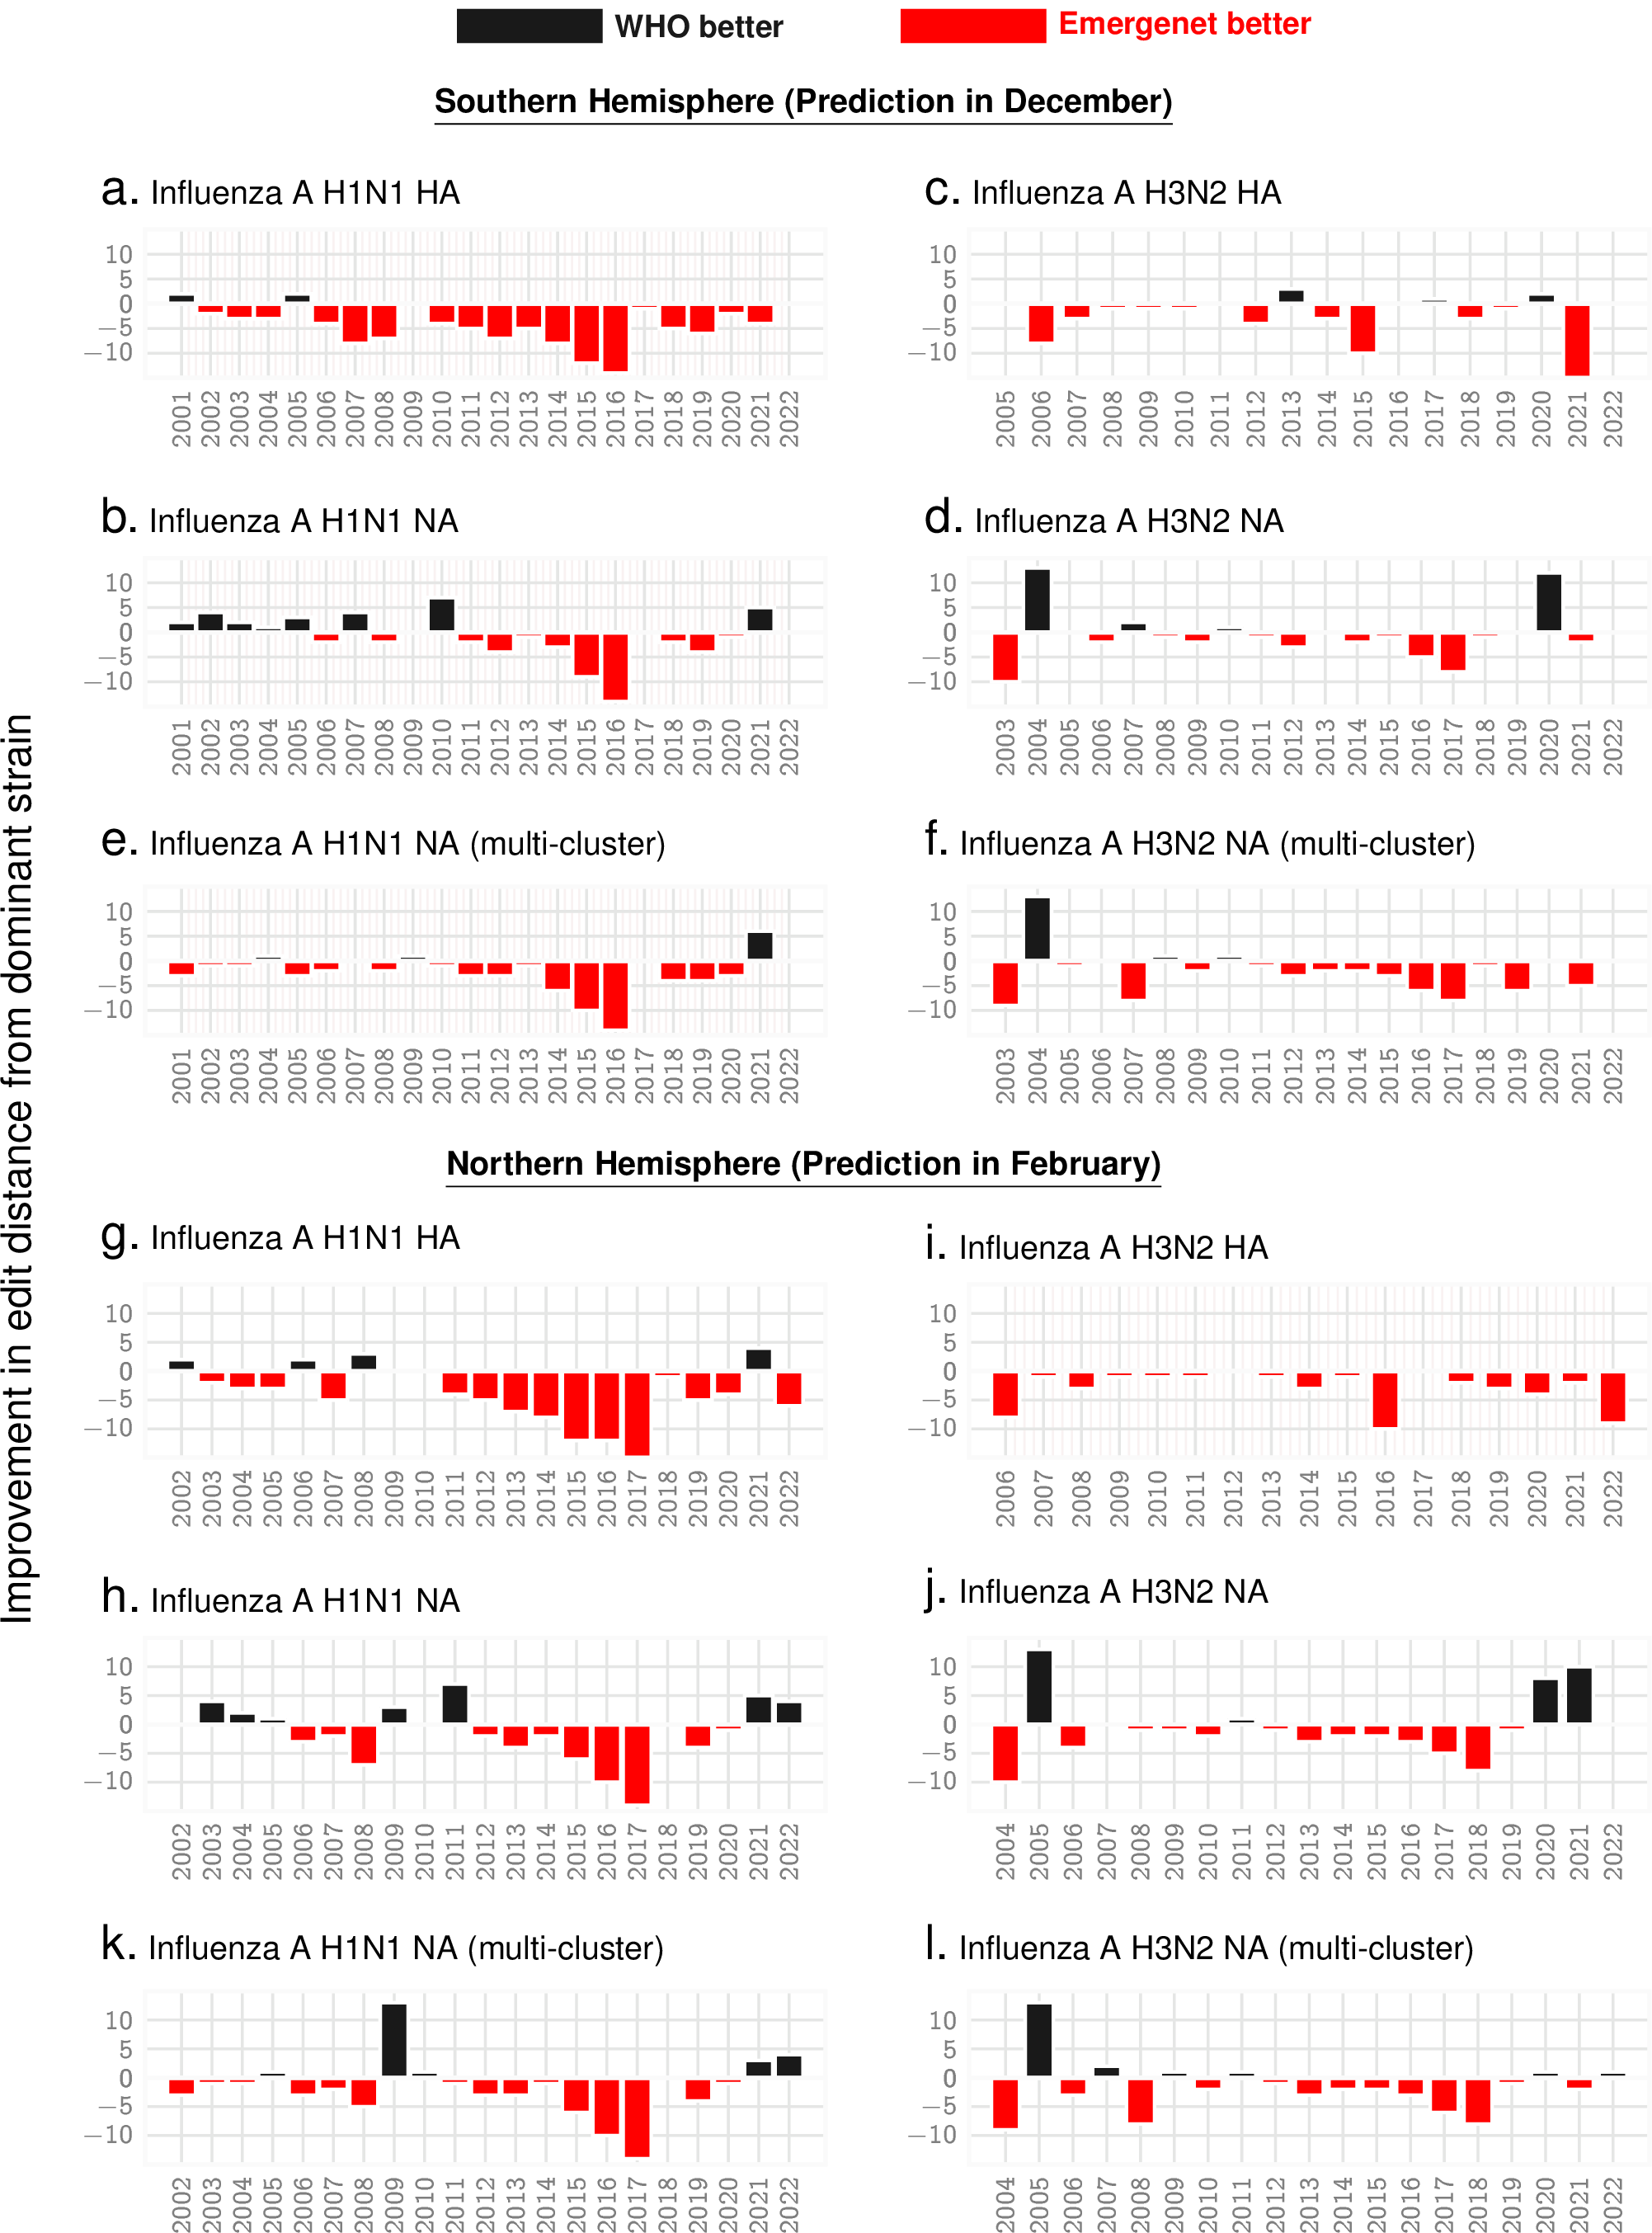
\includegraphics[width=0.975\textwidth]{Figures/seasonalpred_both.tex}
   \fi
   \captionN{\textbf{Seasonal predictions for Influenza A.} Relative out-performance of \qnet predictions against WHO recommendations for H1N1 and H3N2 sub-types for the HA and NA coding sequences over the both hemispheres. The negative bars (red) indicate the reduced edit distance between the predicted sequence and the actual dominant strain that emerged that year. Note that the recommendations for the north are given in February, while that for the south are given at the previous December, keeping in mind that the flu season in the south begins a few months early (e.g. for the 2021-2022 flu season, southern data in the table is labelled `2021' and northern is labelled `2022'). \textbf{Panels e, f, k, l} show further possible improvement in NA predictions if we return three recommendations instead of one each year.}\label{figseasonal}
\end{figure*}
\else
\refstepcounter{figure}\label{figseasonal}
\fi
%#############################################
%#############################################
%#############################################
%#############################################
\ifFIGS
\begin{figure*}[!ht]
  \tikzexternalenable
  \tikzsetnextfilename{figpred}
  \centering
 \tikzXtrue
  \iftikzX 
   \begin{tikzpicture}[font=\sffamily\fontsize{10}{9}\selectfont]
    \def\RFILE{Figures/plotdata/fulldataframe.csv}
  \def\WDT{4.10in}
  \def\HGT{4.35in}
  \def\WDTs{1.6in}
  \def\HGTs{1.6in}
  \def\OPC{.2}
  \def\XFT{-.765in}
\def\TEXTCOLA{black!50}
\def\MCOL{DodgerBlue1!60}
\def\COLBLUE{DodgerBlue3}
\def\DCOL{black}
\def\TXTSZ{6}
\def\GGCOL{black!15}
      \def\FCOL{DarkOrange1!50}
      \def\FCOLA{DarkOrange2!50}
  \def\AXISCOL{black!15}

  \coordinate (Z) at (0,0);
    \node[] (A) at (Z) {
  \begin{tikzpicture}[anchor=center]

  \pgfplotsset{
    discard if/.style 2 args={
      x filter/.append code={
        \edef\tempa{\thisrow{#1}}
        \edef\tempb{#2}
        \ifx\tempa\tempb
        \def\pgfmathresult{inf}
        \fi
      }
    },
    discard if not/.style 2 args={
      x filter/.append code={
        \edef\tempa{\thisrow{#1}}
        \edef\tempb{#2}
        \ifx\tempa\tempb
        \else
        \def\pgfmathresult{inf}
        \fi
      }
    },
    % define the style of the `nodes near coords' that should be shown
    % above the point
    nodes near coords above style/.style={
      font=\bf\fontsize{\TXTSZ}{5}\selectfont,
      text=\TEXTCOLA,
      nodes near coords style={
        anchor=south west,yshift=.07in,
      },
    },
    % define the style of the `nodes near coords' that should be shown
    % above the point
    nodes near coords axove style/.style={
      font=\bf\fontsize{\TXTSZ}{5}\selectfont,
      text=\TEXTCOLA,
      nodes near coords style={
        anchor=south east,yshift=.02in,
      },
    },
    % define the style of the `nodes near coords' that should be shown
    % above the point
    nodes near coords belox style/.style={
      font=\bf\fontsize{\TXTSZ}{5}\selectfont,
      text=\TEXTCOLA,
      nodes near coords style={
        anchor=north west,yshift=.0in,
      },
    },
    % define the style of the `nodes near coords' that should be shown
    % above the point
    nodes near coords beloxx style/.style={
      font=\bf\fontsize{\TXTSZ}{5}\selectfont,
      text=\TEXTCOLA,
      nodes near coords style={
        anchor=north west,yshift=.02in,
      },
    },
    % define the style of the `nodes near coords' that should be shown
    % below the point
    nodes near coords below style/.style={
       font=\bf\fontsize{\TXTSZ}{5}\selectfont,
      text=\TEXTCOLA,
     nodes near coords style={
        anchor=north, yshift=-.05in, xshift=-.1in,
      },
    },
    % define the style of the `nodes near coords' that should be shown
    % below the point
    nodes near coords right style/.style={
        font=\bf\fontsize{\TXTSZ}{5}\selectfont,
      text=\TEXTCOLA,
    nodes near coords style={
        anchor=west,xshift=.02in,
      },
    },
    % define the style of the `nodes near coords' that should be shown
    % below the point
    nodes near coords left style/.style={
       font=\bf\fontsize{\TXTSZ}{5}\selectfont,
       text=\TEXTCOLA,
    nodes near coords style={
        anchor=east,
        xshift=-.02in,yshift=-.04in,
      },
    },
    % define the style of the `nodes near coords' that should be shown
    % below the point
    nodes near coords null style/.style={
         font=\bf\fontsize{\TXTSZ}{5}\selectfont,
      text=\TEXTCOLA,
   nodes near coords style={
        anchor=west,text opacity=0,
      },
    },
  }



    \begin{axis}[enlargelimits=false,scale only axis=true,
      axis line style={\AXISCOL, opacity=1,thin, rounded corners=0pt},
      grid style={thin,\GGCOL},
      grid=both,
      enlargelimits=0.01, 
      width=\WDT, 
      height=\HGT,
      scaled ticks = false,
      x tick label style={yshift=-.05in,/pgf/number format/fixed,
        /pgf/number format/1000 sep = %\thinspace % Optional if you want to replace comma as the 1000 separator 
      },yticklabel style={/pgf/number format/fixed,
        /pgf/number format/precision=2},,xticklabel style={/pgf/number format/fixed,
        /pgf/number format/precision=2},
      major tick length=0pt,
      yticklabel style={xshift=-.015in}, nodes near coords,
      point meta=explicit symbolic,
      table/meta=strain,      axis on top=false,
      ymax=7.6,      xlabel={geometric mean of HA and NA \qdist },ylabel={IRAT emergence score},xlabel style={yshift=-.1in},ylabel style={yshift=-.15in},
%axis x line=bottom,
%axis y line=left,
ymin=2.65,
ymax=7.7,
      ]



      \addplot[smooth, ultra thick,draw=white, opacity=1,mark=none,
      nodes near coords null style, ] table[col sep=comma,
      x=geometric mean of Edistances,y=pred_GM] \RFILE;

      \addplot[nodes near coords null style,forget plot,
      name path=UB,smooth, ultra thick,
      mark=none,draw=none ] table[col sep=comma,
      x=geometric mean of Edistances,y=ub_GM] \RFILE;
      
      \addplot[nodes near coords null style,
      forget plot, name path=LB,smooth,
      ultra thick, mark=none,draw=none ] table[col sep=comma,
      x=geometric mean of Edistances,y=lb_GM] \RFILE;
      
      \addplot[nodes near coords null style,
      forget plot,\FCOLA,opacity=1] fill between[of=LB and UB];
      
      
      \addplot[only marks, mark=*,
      mark options={fill=black,fill=\MCOL,draw=\DCOL,scale=1.5},
      nodes near coords below style,      
      discard if={strain}{A/Shanghai/02/2013},
      discard if={strain}{A/Indiana/08/2011},
      discard if={strain}{A/Ohio/13/2017},
      discard if={strain}{A/Hong Kong/125/2017},
      discard if={strain}{A/Sichuan/06681/2021},
      discard if={strain}{A/California/62/2018},
      discard if={strain}{A/Bangladesh/0994/2011},
      discard if={strain}{A/Anhui-Lujiang/39/2018},
      discard if={strain}{A/chicken/Tennessee/17-007431-3/2017},
      discard if={strain}{A/chicken/Tennessee/17-007147-2/2017},
      discard if={strain}{A/Yunnan/14564/2015},
      discard if={strain}{A/Astrakhan/3212/2020},
      discard if={strain}{A/canine/Illinois/12191/2015},
      discard if={strain}{A/gyrfalcon/Washington/41088/2014},
      discard if={strain}{A/turkey/Indiana/1573-2/2016},
      discard if={strain}{A/American wigeon/South Carolina/AH0195145/2021},
      discard if={strain}{A/Jiangxi-Donghu/346/2013},
      %discard if={strain}{A/swine/Shandong/1207/2016},
      discard if={strain}{A/American green-winged teal/Washington/1957050/2014},
      discard if={strain}{A/Northern pintail/Washington/40964/2014},
      discard if={strain}{A/Netherlands/219/2003} ]
      table[x=geometric mean of Edistances,
      y=IRAT Emergence Estimate,col sep=comma] \RFILE;


      \pgfplotsinvokeforeach {
        A/canine/Illinois/12191/2015,
        A/Netherlands/219/2003%
      } {
        \addplot+ [only marks,
        mark=*,
        mark options={fill=\MCOL,draw=\DCOL,scale=1.5},
        nodes near coords below style,
        forget plot,text=black,
        nodes near coords above style,
        discard if not={strain}{#1},
        ] table[x=geometric mean of Edistances,
        y=IRAT Emergence Estimate,col sep=comma]\RFILE;
      }


      \pgfplotsinvokeforeach {
        A/turkey/Indiana/1573-2/2016,
        A/American green-winged teal/Washington/1957050/2014,
        A/chicken/Tennessee/17-007147-2/2017,
        A/Northern pintail/Washington/40964/2014,
        A/American wigeon/South Carolina/AH0195145/2021,
        A/chicken/Tennessee/17-007431-3/2017,A/Astrakhan/3212/2020,
        A/Yunnan/14564/2015%
      } {
        \addplot+ [only marks,
        mark=*,mark options={fill=black,fill=\MCOL,draw=\DCOL,scale=1.5},
        forget plot,
        nodes near coords right style,
        discard if not={strain}{#1},
        ] table[x=geometric mean of Edistances,
        y=IRAT Emergence Estimate,col sep=comma]\RFILE;
      }

      \pgfplotsinvokeforeach {
       % A/swine/Shandong/1207/2016,
        A/Indiana/08/2011,
        A/Shanghai/02/2013,
        A/Hong Kong/125/2017,
        A/Sichuan/06681/2021,
        A/Bangladesh/0994/2011,
        A/Anhui-Lujiang/39/2018,
        A/California/62/2018% 
      } {
        \addplot+ [only marks,
        mark=*,mark options={fill=black,fill=\MCOL,draw=\DCOL,scale=1.50},
        forget plot,
        nodes near coords left style,
        discard if not={strain}{#1},
        ] table[x=geometric mean of Edistances,
        y=IRAT Emergence Estimate,col sep=comma]\RFILE;
      }

      \pgfplotsinvokeforeach {
        A/Ohio/13/2017,
      } {
        \addplot+ [only marks,
        mark=*,mark options={fill=black,fill=\MCOL,draw=\DCOL,scale=1.50},
        forget plot,
        nodes near coords axove style,
        discard if not={strain}{#1},
        ] table[x=geometric mean of Edistances,
        y=IRAT Emergence Estimate,col sep=comma]\RFILE;
      }

     \pgfplotsinvokeforeach {
 A/gyrfalcon/Washington/41088/2014,
      } {
        \addplot+ [only marks,
        mark=*,mark options={fill=black,fill=\MCOL,draw=\DCOL,scale=1.50},
        forget plot,
        nodes near coords belox style,
        discard if not={strain}{#1},
        ] table[x=geometric mean of Edistances,
        y=IRAT Emergence Estimate,col sep=comma]\RFILE;
      }
     \pgfplotsinvokeforeach {A/Jiangxi-Donghu/346/2013,
      } {
        \addplot+ [only marks,
        mark=*,mark options={fill=black,fill=\MCOL,draw=\DCOL,scale=1.50},
        forget plot,
        nodes near coords beloxx style,
        discard if not={strain}{#1},
        ] table[x=geometric mean of Edistances,
        y=IRAT Emergence Estimate,col sep=comma]\RFILE;
      }

      \node [anchor=center,font=\bf\sffamily\fontsize{6}{6}\selectfont] at (axis cs:-0.23,3) {H7N9};
      \node [anchor=center,font=\bf\sffamily\fontsize{6}{6}\selectfont] at (axis cs:-0.16,3.265) {H7N9};
  \node [anchor=center,font=\bf\sffamily\fontsize{6}{6}\selectfont] at (axis cs:-0.31,5.2) {H5N6};
  \node [anchor=center,font=\bf\sffamily\fontsize{6}{6}\selectfont] at (axis cs:-0.315,4.45) {H7N7};
 \node [anchor=center,font=\bf\sffamily\fontsize{6}{6}\selectfont] at (axis cs:-0.296,4.25) {H5N1};
  \node [anchor=center,font=\bf\sffamily\fontsize{6}{6}\selectfont] at (axis cs:-0.296,3.27) {H7N8};
   \node [anchor=center,font=\bf\sffamily\fontsize{6}{6}\selectfont] at (axis cs:-0.31,3.6) {H5N1};
  \node [anchor=center,font=\bf\sffamily\fontsize{6}{6}\selectfont] at (axis cs:-0.26,3.8) {H5N2};
 \node [anchor=center,font=\bf\sffamily\fontsize{6}{6}\selectfont] at (axis cs:-0.25,4.6) {H5N8};
   \node [anchor=center,font=\bf\sffamily\fontsize{6}{6}\selectfont] at (axis cs:-0.245,4.2) {H5N8};
      \node [anchor=center,font=\bf\sffamily\fontsize{6}{6}\selectfont] at (axis cs:-0.225,4.3) {H10N8};
      \node [anchor=center,font=\bf\sffamily\fontsize{6}{6}\selectfont] at (axis cs:-0.19,5.8) {H9N2};
      \node [anchor=center,font=\bf\sffamily\fontsize{6}{6}\selectfont] at (axis cs:-0.15,5.42) {H5N6};
      \node [anchor=center,font=\bf\sffamily\fontsize{6}{6}\selectfont] at (axis cs:-0.08,3.7) {H3N2};
      \node [anchor=center,font=\bf\sffamily\fontsize{6}{6}\selectfont] at (axis cs:-0.067,5.8) {H1N2};
      \node [anchor=center,font=\bf\sffamily\fontsize{6}{6}\selectfont] at (axis cs:-0.055,6.2) {H9N2};
      \node [anchor=center,font=\bf\sffamily\fontsize{6}{6}\selectfont] at (axis cs:-0.06,7.5) {H1N1};
      \node [anchor=center,font=\bf\sffamily\fontsize{6}{6}\selectfont] at (axis cs:-0.06,5.2) {H5N1};
      \node [anchor=center,font=\bf\sffamily\fontsize{6}{6}\selectfont] at (axis cs:-0.0375,6.6) {H3N2};
      \node [anchor=center,font=\bf\sffamily\fontsize{6}{6}\selectfont] at (axis cs:-0.08,6.55) {H7N9};
      \node [anchor=center,font=\bf\sffamily\fontsize{6}{6}\selectfont] at (axis cs:-0.02,6.25) {H7N9};
      \node [anchor=center,font=\bf\sffamily\fontsize{6}{6}\selectfont] at (axis cs:-0.02,5.85) {H3N2};


            \node [text=\COLBLUE,anchor=north west,fill=white,align=left,font=\bf\sffamily\fontsize{8}{9}\selectfont] (LLEQ1) at (axis cs:-.25,6.5) {$R = 0.703$\\p-value\\$0.00026$};


    \end{axis}
  \end{tikzpicture}};
\node[anchor=north west] (B) at ([xshift=\XFT]A.north east) {
      \def\RFILE{Figures/plotdata/fulldataframe_sortE.csv}

  \begin{tikzpicture}[anchor=center]
\begin{axis}[enlargelimits=false,scale only axis=true,
      axis line style={\AXISCOL, opacity=1,thin, rounded corners=0pt},
      grid style={thin,\GGCOL},
      grid=both,
      enlargelimits=0.015, 
      width=\WDTs, 
      height=\HGTs,
      scaled ticks = false,
      x tick label style={yshift=-.05in,/pgf/number format/fixed,
        /pgf/number format/1000 sep = %\thinspace % Optional if you want to replace comma as the 1000 separator 
      },yticklabel style={/pgf/number format/fixed,
        /pgf/number format/precision=2},,xticklabel style={/pgf/number format/fixed,
        /pgf/number format/precision=2},
      major tick length=0pt,
      yticklabel style={xshift=-.015in}, %nodes near coords,
      %point meta=explicit symbolic,
      %table/meta=strain,
      axis on top=false,
      ymax=7.6,
      xmin=3.25,xmax=6.8,      xlabel={predicted emergence score},
      ylabel={IRAT emergence score},,xlabel style={yshift=-.05in,xshift=0in},ylabel style={yshift=-.225in},
      ]

        \addplot[smooth, only marks, mark=*, mark options={fill=white,scale=.8},, opacity=1,mark=none, ] table[col sep=comma,
      y=IRAT Emergence Estimate,x=Emergenet emergence estimate] \RFILE;

      \addplot[smooth, ultra thick,draw=white, opacity=1,mark=none, ] table[col sep=comma,
      y=pred_E,x=Emergenet emergence estimate] \RFILE;

      \addplot[forget plot,
      name path=UB,smooth, ultra thick,
      mark=none,draw=none ] table[col sep=comma,
      y=ub_E,x=Emergenet emergence estimate] \RFILE;
      
      \addplot[forget plot, name path=LB,smooth,
      ultra thick, mark=none,draw=none ] table[col sep=comma,
      y=lb_E,x=Emergenet emergence estimate] \RFILE;
      
      \addplot[forget plot,\FCOL,opacity=1] fill between[of=LB and UB];

      \node [text=\COLBLUE,anchor=north west,fill=white] (LLEQ1) at (axis cs:3.3,7) {OLS fit: $y=x$};

        \node [text=\COLBLUE,anchor=north west,fill=white,align=left,font=\bf\sffamily\fontsize{8}{9}\selectfont] (LLEQ1) at (axis cs:5,4) {$R = 0.81$\\p-value\\$4.7\times 10^{-6}$};

\end{axis}
  \end{tikzpicture}
  };


\node[anchor=south west] (C) at ([xshift=\XFT]A.south east) {
      \def\RFILE{Figures/plotdata/fulldataframe_sortI.csv}

  \begin{tikzpicture}[anchor=center]
\begin{axis}[enlargelimits=false,scale only axis=true,
      axis line style={\AXISCOL, opacity=1,thin, rounded corners=0pt},
      grid style={thin,\GGCOL},
      grid=both,
      enlargelimits=0.015, 
      width=\WDTs, 
      height=\HGTs,
      scaled ticks = false,
      x tick label style={yshift=-.05in,/pgf/number format/fixed,
        /pgf/number format/1000 sep = %\thinspace % Optional if you want to replace comma as the 1000 separator 
      },yticklabel style={/pgf/number format/fixed,
        /pgf/number format/precision=2},,xticklabel style={/pgf/number format/fixed,
        /pgf/number format/precision=2},
      major tick length=0pt,
      yticklabel style={xshift=-.015in}, %nodes near coords,
      %point meta=explicit symbolic,
      %table/meta=strain,
      axis on top=false,
      ymax=7.6,      xmin=3.75,xmax=6.8,
      xlabel={predicted impact score},
      ylabel={IRAT impact score},,xlabel style={yshift=-.05in,xshift=0in},ylabel style={yshift=-.225in},
      ]

      
      \addplot[smooth, only marks, mark=*, mark options={fill=white,scale=.8},, opacity=1,mark=none, ] table[col sep=comma,
      y=IRAT Impact Estimate,x=Emergenet impact estimate] \RFILE;

      \addplot[smooth, ultra thick,draw=white, opacity=1,mark=none, ] table[col sep=comma,
      y=pred_I,x=Emergenet impact estimate] \RFILE;

      \addplot[forget plot,
      name path=UB,smooth, ultra thick,
      mark=none,draw=none ] table[col sep=comma,
      y=ub_I,x=Emergenet impact estimate] \RFILE;
      
      \addplot[forget plot, name path=LB,smooth,
      ultra thick, mark=none,draw=none ] table[col sep=comma,
      y=lb_I,x=Emergenet impact estimate] \RFILE;
      
      \addplot[forget plot,\FCOL,opacity=1] fill between[of=LB and UB];


      \node [text=\COLBLUE,anchor=north west,fill=white] (LLEQ1) at (axis cs:3.7,7) {OLS fit: $y=x$};
        \node [text=\COLBLUE,anchor=north west,fill=white,align=left,font=\bf\sffamily\fontsize{8}{9}\selectfont] (LLEQ1) at (axis cs:5.25,4.5) {$R = 0.77$\\p-value\\$3.3\times 10^{-5}$};
\end{axis}
  \end{tikzpicture}
  };


  \node[anchor=north west] (W) at ([yshift=-.4in]A.south west) {
    \begin{tikzpicture}[font=\bf\sffamily\fontsize{8}{8}\selectfont]
 \begin{scope}
 \clip (-3.4in,1.25in) rectangle (3.35in,-1in);
\node[anchor=center] (A11) at (0,0) {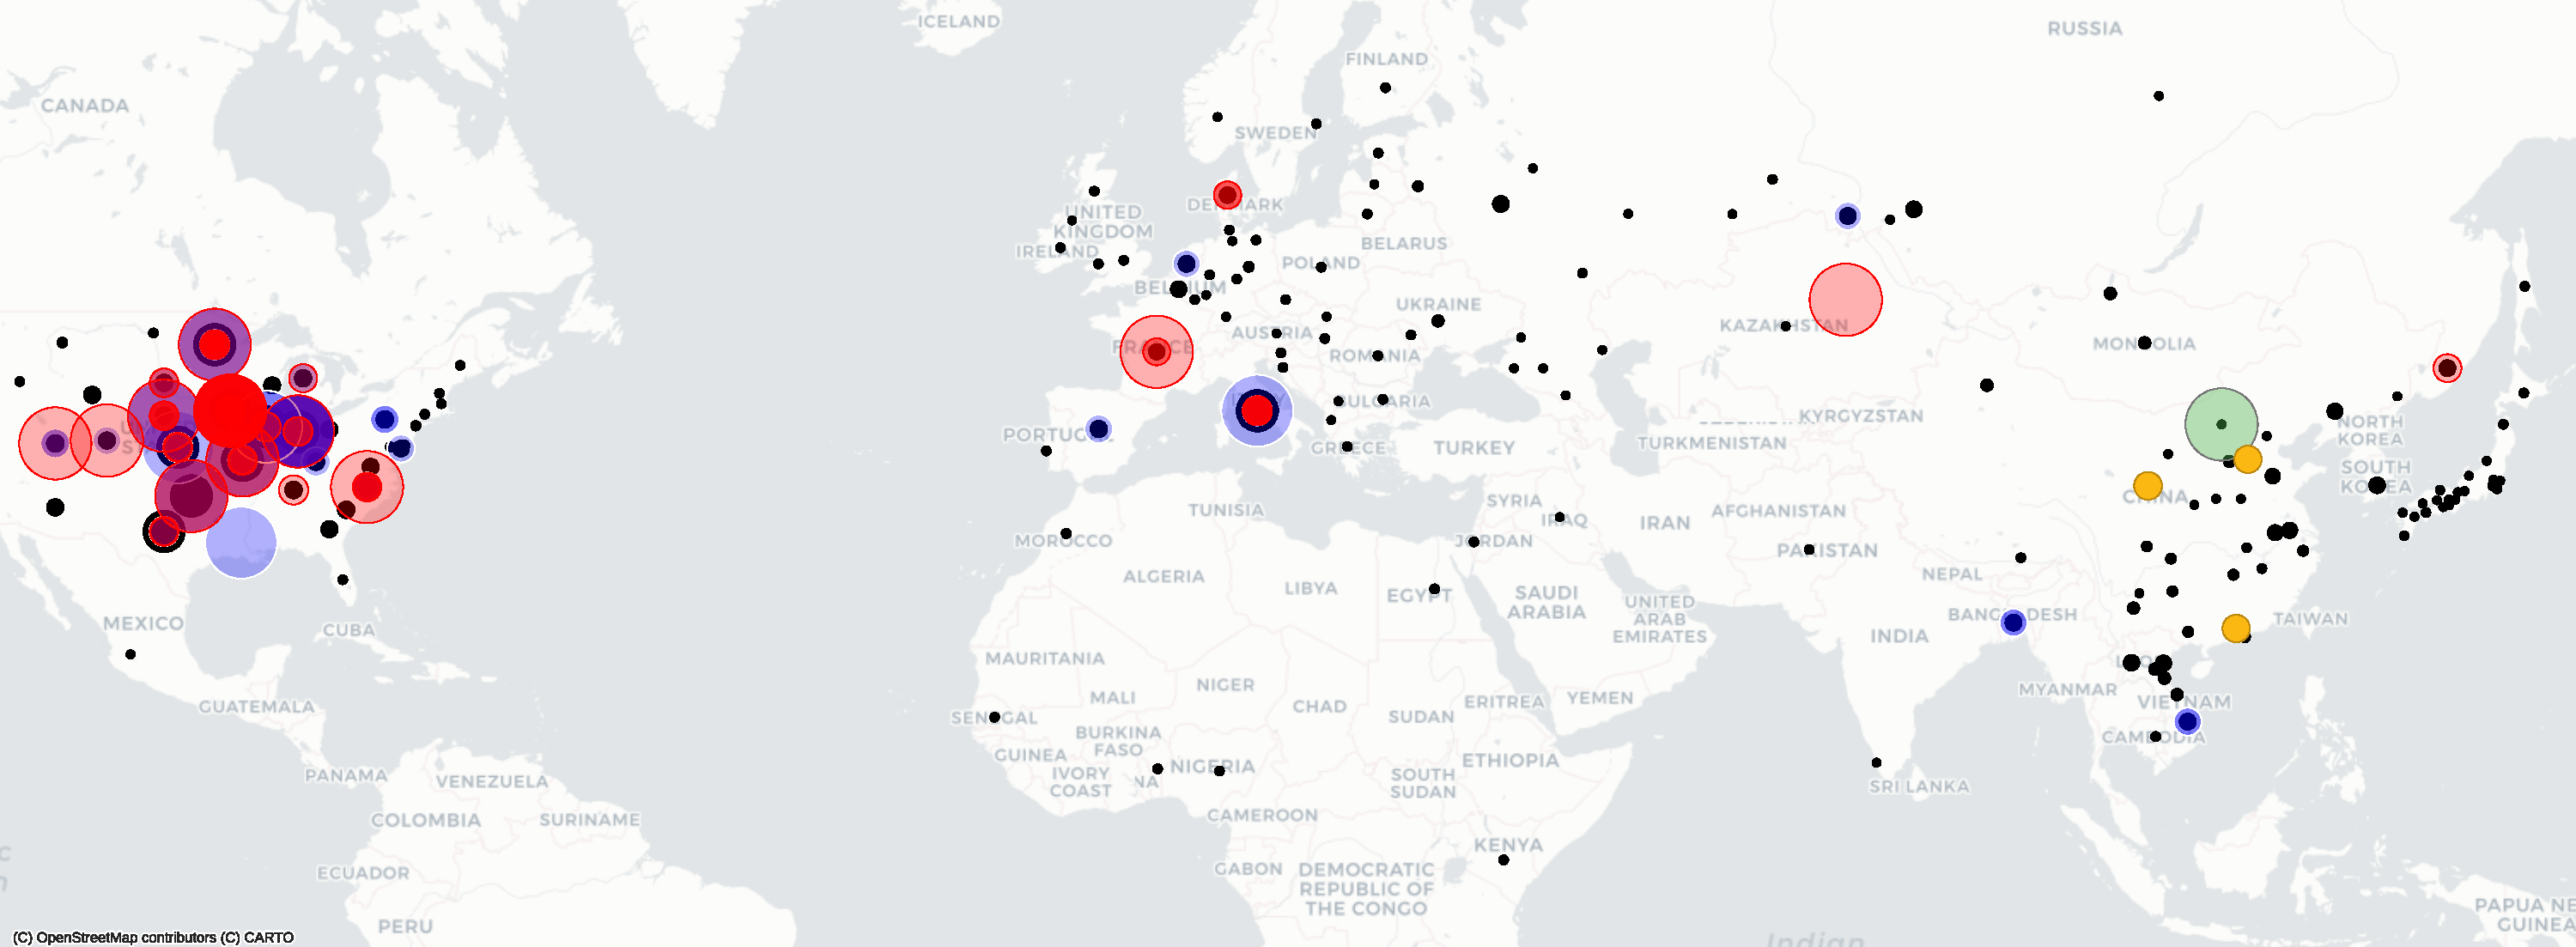
\includegraphics[width=\textwidth]{Figures/bionorad}};
\end{scope}

%7.5 7.2 6.8 <6
\def\TEXTCOLA{black!60}

\node[circle,fill=white,inner sep=1pt,text width=.195in,draw=\TEXTCOLA,label={[text=gray,align=center,font=\bf\sffamily\fontsize{7}{8}\selectfont]90:Geometric mean of\\predicted impact and emergence  scores}] (C1) at ([xshift=-1.65in,yshift=.9in]A11.center) {};
\node [anchor=west,align=left,text=\TEXTCOLA,] (LL1) at ([xshift=.1in]C1.center) {$7.5$};
\node[circle,fill=white,text width=.175in,draw=\TEXTCOLA,inner sep=1pt,,anchor=north,text=\TEXTCOLA] (C1) at ([yshift=-.1in]C1.south) {};
\node[circle,fill=white,text width=.11in,draw=\TEXTCOLA,inner sep=1pt,,anchor=north,text=\TEXTCOLA] (C1) at ([yshift=-.1in]C1.south) {};
\node[circle,fill=white,text width=.075in,inner sep=1pt,draw=\TEXTCOLA,,anchor=north,text=\TEXTCOLA] (C1) at ([yshift=-.1in]C1.south) {};
\node[circle,fill=white,inner sep=1pt,text width=.005in,draw=\TEXTCOLA,,anchor=north,text=\TEXTCOLA] (C1) at ([yshift=-.12in]C1.south) {};
\node [anchor=north,align=left,text=\TEXTCOLA] (LL1) at ([yshift=-.15in]LL1.south) {$7.2$};
\node [anchor=north,align=left,text=\TEXTCOLA] (LL1) at ([yshift=-.11in]LL1.south) {$6.8$};
\node [anchor=north,align=left,text=\TEXTCOLA] (LL1) at ([yshift=-0.06in]LL1.south) {$6.7$};
\node [anchor=north,align=left,text=\TEXTCOLA] (LL1) at ([yshift=-0.03in]LL1.south) {$6.0$};

\node[font=\sffamily\fontsize{6}{6}\selectfont,align=center,fill=Red1!60,text width=.25in,anchor=north,xshift=-.05in,yshift=-.351in,label={[font=\bf\sffamily\fontsize{7}{8}\selectfont,xshift=.1in,text=gray]90:subtypes of high-risk strains}] (X1) at (C1.south) {H1N1};
\node[font=\sffamily\fontsize{6}{6}\selectfont,align=center,text=white,fill=Blue1!60,text width=.25in,anchor=north,xshift=0in,yshift=-.051in] (X2) at (X1.south) {H3N2};
\node[font=\sffamily\fontsize{6}{6}\selectfont,align=center,text=white,fill=Yellow3!70!black,text width=.25in,anchor=west,xshift=0.02in,yshift=0in] (X1) at (X1.east) {H5N2};
\node[font=\sffamily\fontsize{6}{6}\selectfont,align=center,fill=Green4!50,text width=.25in,anchor=north,xshift=0in,yshift=-.051in] (X1) at (X1.south) {H7N9};


\node [] (LD1) at ([yshift=.5in,xshift=1in]A11.center) {};
\draw [] (LD1)node [right,above,align=center,font=\bf\sffamily\fontsize{5}{5}\selectfont] {A/chicken/Bulgaria/221\_20VIR1725-1/2020\\(emergence: 6.4, impact: 8.8)}  -- ++(-.4in,0in) -- ++(-.2in,-.19in) ;




\node [text=Red1] (LD2) at ([yshift=.47in,xshift=-.25in]A11.east) {};
\draw [] (LD2) node [xshift=-.2in,right,above,align=right,font=\bf\sffamily\fontsize{5}{5}\selectfont,xshift=-.25in] {A/Chicken/Hebei/1011/2021\\(emergence: 6.7, impact: 7.7)}  -- ++(-.4in,0in) -- ++(-.2in,-.2in) ;


\node [text=Red1] (LD3) at ([yshift=.85in,xshift=-2.05in]A11.east) {};
\draw [] (LD3) node [right,above,align=center,font=\bf\sffamily\fontsize{5}{5}\selectfont,xshift=-.25in] {A/Camel/Inner\_Mongolia/XL/2020\\(emergence: 6.8, impact: 6.7)}  -- ++(.4in,0in) -- ++(.6in,-.6in) ;



\node [text=Red1] (LD4) at ([yshift=-.25in,xshift=.75in]A11.west) {};
\draw [] (LD4) node [right,above,xshift=.65in,align=center,font=\bf\sffamily\fontsize{5}{5}\selectfont,xshift=-.25in] {A/swine/Missouri/A02524711/2020\\(emergence: 6.8, impact: 6.7)}  -- ++(-.4in,0in) -- ++(.3in,.3in) ;

\end{tikzpicture}
    };

  
\node[anchor=south west] (LA) at (A.north west) {{\Large a.} \bf Predicted emergence risk vs published IRAT scores};
\node[anchor=south west,align=left] (LB) at ([xshift=0in]B.north west) {{\Large b.} \bf Estimating emergence};
\node[anchor=south west] (LC) at ([xshift=.1in]C.north west) {{\Large c.} \bf Estimating  impact};
\node[anchor=south west] (LW) at ([xshift=.1in]W.north west) {{\Large d.} \bf Global prediction of IRAT scored for all \infl sequences collected since 2020};


\end{tikzpicture}
    
   \else 
   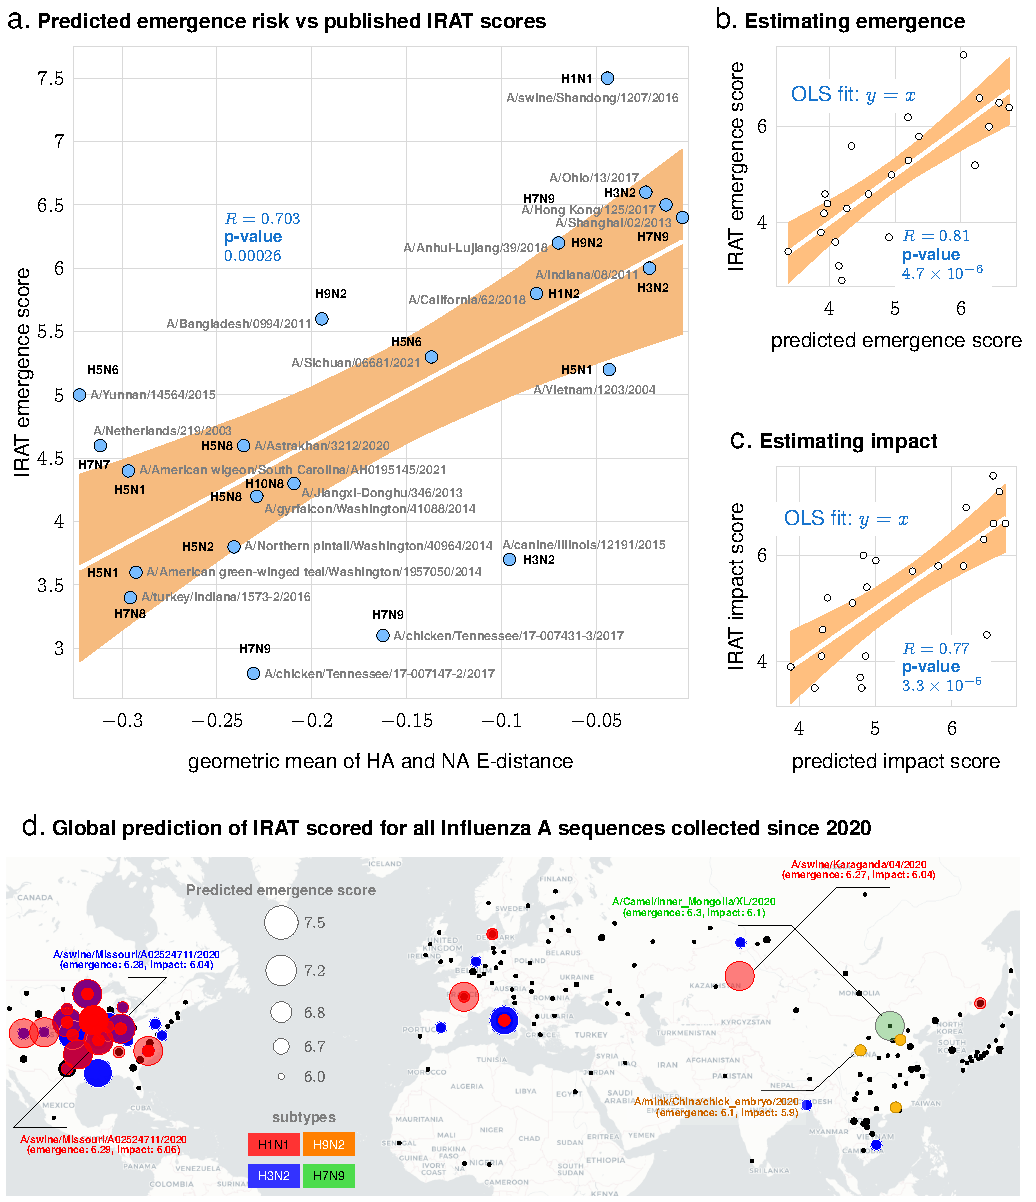
\includegraphics[width=\textwidth]{Figures/External/figpred}
   \fi
  \captionN{\textbf{IRAT emergence risk vs. q-distance}. There is an approximate linear relationship between average q-distance from human circulating strains (averaged across both HA and NA) and IRAT emergence risk grade. % Note that IRAT has released results for 23 strains to date, but only 15 are plotted on the graph. This is because the strains not pictured have less than 30 human strains of the same sub-type, so a sufficiently representative \qnet could not be trained.
  }\label{figirat}
\end{figure*}
\else
\refstepcounter{figure}\label{figirat}
\fi
%#############################################
%#############################################
\ifFIGS

\begin{table}[!ht]\centering
\captionN{Influenza A Strains Evaluated by IRAT and Corresponding \qnet Computed Risk Scores}\label{irattab}

\sffamily\fontsize{7}{8}\selectfont

\begin{tabular}{L{1.25in}|L{.35in}|L{.3in}|L{.3in}|L{.3in}|L{.35in}|L{.35in}|L{.35in}|L{.35in}|L{.32in}|L{.3in}|L{.3in}}\hline
Influenza Virus & Subype & IRAT Date &IRAT Emergence Score &IRAT Impact Score &HA Sample &NA Sample &HA \erisk & NA \erisk &Geom. Mean&\qnet Emergence Score&\qnet Impact Score \\\hline
 A/swine/Shandong/1207/2016 &H1N1& Jul  2020 &7.5&6.9&1000&1000&-0.0941&-0.0205&0.0440&6.0&6.2\\\hline
 A/Ohio/13/2017 &H3N2& Jul  2019 &6.6&5.8&1000&1000&-0.0184&-0.0306&0.0238&6.3&6.2\\\hline
 A/Hong  Kong/125/2017 &H7N9& May  2017 &6.5&7.5&437&437&-0.0296&-0.0058&0.0131&6.6&6.5\\\hline
 A/Shanghai/02/2013 &H7N9& Apr  2016 &6.4&7.2&178&178&-0.0055&-0.0036&0.0044&6.7&6.6\\\hline
 A/Anhui-Lujiang/39/2018 &H9N2& Jul  2019 &6.2&5.9&31&30&-0.0290&-0.1681&0.0698&5.2&5.0\\\hline
 A/Indiana/08/2011 &H3N2& Dec  2012 &6.0&4.5&1000&1000&-0.0523&-0.0091&0.0218&6.4&6.5\\\hline
 A/California/62/2018 &H1N2& Jul  2019 &5.8&5.7&55&55&-0.1089&-0.0610&0.0815&5.4&5.5\\\hline
 A/Bangladesh/0994/2011$^{\star\star\star}$ &H9N2& Feb  2014 &5.6&5.4&&&-0.2078&-0.1823&0.1947&4.3&4.9\\\hline
 A/Sichuan/06681/2021 &H5N6& Oct  2021 &5.3&6.3&45&45&-0.3616&-0.0518&0.1369&5.2&6.4\\\hline
 A/Vietnam/1203/2004 &H5N1& Nov  2011 &5.2&6.6&258&246&-0.1673&-0.0111&0.0430&6.2&6.7\\\hline
 A/Yunnan/14564/2015$^{\star\star}$ &H5N6& Apr  2016 &5.0&6.6&344&331&-0.3482&-0.2987&0.3225&4.9&6.5\\\hline
 A/Astrakhan/3212/2020$^{\star\star}$ &H5N8& Mar  2021 &4.6&5.2&381&365&-0.1603&-0.3472&0.2359&3.9&4.4\\\hline
 A/Netherlands/219/2003 &H7N7& Jun  2012 &4.6&5.8&46&46&-0.2757&-0.3521&0.3115&4.6&5.8\\\hline
 A/American  wigeon/South  Carolina/AH0195145/2021 &H5N1& Mar  2022 &4.4&5.1&335&323&-0.1722&-0.5114&0.2967&4.0&4.7\\\hline
 A/Jiangxi-Donghu/346/2013$^{\star\star\star}$ &H10N8& Feb  2014 &4.3&6.0&&&-0.2088&-0.2101&0.2094&4.3&4.8\\\hline
 A/gyrfalcon/Washington/ 41088/2014$^{\star\star}$ &H5N8& Mar  2015 &4.2&4.6&341&328&-0.1532&-0.3424&0.2290&3.9&4.3\\\hline
 A/Northern  pintail/ Washington/40964/2014$^{\star\star}$ &H5N2& Mar  2015 &3.8&4.1&341&328&-0.1529&-0.3799&0.2410&3.9&4.3\\\hline
 A/canine/Illinois/12191/2015 &H3N2& Jun  2016 &3.7&3.7&1000&1000&-0.0607&-0.1509&0.0957&4.9&4.8\\\hline
 A/American  green-winged  teal /Washington/1957050/2014 &H5N1& Mar 2015 &3.6&4.1&326&314&-0.1911&-0.4482&0.2927&4.1&4.9\\\hline
 A/turkey/Indiana/1573-2/2016$^{\star\star}$ &H7N8& Jul  2017 &3.4&3.9&495&494&-0.1130&-0.7738&0.2957&3.4&3.9\\\hline
 A/chicken/Tennessee/17-007431-3/2017 &H7N9& Oct  2017 &3.1&3.5&496&495&-0.1027&-0.2569&0.1624&4.1&4.2\\\hline
 A/chicken/Tennessee/17-007147-2/2017 &H7N9& Oct  2017 &2.8&3.5&496&495&-0.2095&-0.2541&0.2307&4.2&4.8\\\hline
% A/duck/New  York/1996 $^\star$&H1N1& Nov  2011 &2.3&2.4&1000&1000&-1&-1&-1&-1&-1\\\hline
 \end{tabular}
\flushleft

\fontsize{8}{8}\selectfont
$^\star$ HA strain is not available for A/duck/New York/1996, so this strain is omitted.\\
$^{\star\star}$ Could not construct a \qnet of human sequence data available for that virus sub-type (less than 30 strains), so we constructed a \qnet using all human strains that match the HA sub-type, i.e. H5NX for H5N6.\\
$^{\star\star\star}$ These strains did not have enough human sequence data to generate a \qnet, even when only considering the HA sub-type. Thus, we estimated the risk score using every \qnet from the other IRAT strains, and took the average among NA and HA. Finally, we took the geometric mean of the resulting NA and HA averages.
\end{table}
\else
\refstepcounter{table}\label{irattab}
\fi
% #############################################
%#############################################
\ifFIGS

\begin{table}[!ht]\centering
\captionN{Influenza A Strains Evaluated by IRAT and Corresponding \qnet Computed Risk Scores}\label{highrisktab}

\bf\sffamily\fontsize{7}{7}\selectfont

\begin{tabular}{L{1.95in}|L{.25in}|L{.60in}|L{.6in}|C{1in}|C{1in}}\hline
strain&subtype& HA  accession & NA  accession & predicted  IRAT  impact & predicted  IRAT  emergence \\
 \rowcolor{Red3!20}A/swine/Missouri/A02524711/2020 &H1N1&EPI1818121&EPI1818122&6.6318&6.7067\\
 \rowcolor{Green3!50}A/Camel/Inner\_Mongolia/XL/2020 &H7N9&EPI2026200&EPI2026202&6.6286&6.7026\\
 \rowcolor{Blue1!30}A/swine/Indiana/A02524710/2020 &H3N2&EPI1818137&EPI1818138&6.6070&6.6757\\
 \rowcolor{Red3!20}A/swine/North\_Carolina/A02479173/2020 &H1N1&EPI1780425&EPI1780426&6.5878&6.6517\\
 \rowcolor{Red3!20}A/swine/Tennessee/A02524414/2022 &H1N1&EPI2149257&EPI2149258&6.5379&6.5893\\
 \rowcolor{Red3!20}A/swine/Minnesota/A02635976/2021 &H1N1&EPI1912208&EPI1912209&6.4841&6.5220\\
 \rowcolor{Blue1!30}A/swine/Chile/VN1401-5054/2020 &H3N2&EPI1974975&EPI1974978&6.4578&6.4891\\
 \rowcolor{Blue1!30}A/swine/Italy/56910/2020 &H3N2&EPI2142217&EPI2142173&6.4537&6.4840\\
 \rowcolor{Blue1!30}A/swine/Minnesota/A02245643/2020 &H3N2&EPI1769178&EPI1769179&6.4370&6.4631\\
 \rowcolor{Red3!20}A/swine/Iowa/A02479005/2020 &H1N1&EPI1777621&EPI1777622&6.4103&6.4297\\
 \rowcolor{Blue1!30}A/swine/Iowa/A02524874/2020 &H3N2&EPI1907838&EPI1907839&6.3836&6.3962\\
 \rowcolor{Red3!20}A/swine/Indiana/A02636638/2022 &H1N1&EPI2153370&EPI2153371&6.3830&6.3954\\
 \rowcolor{Blue1!30}A/swine/Illinois/A02479007/2020 &H3N2&EPI1777629&EPI1777630&6.3769&6.3877\\
 \rowcolor{Blue1!30}A/swine/Spain/44579-1/2020 &H3N2&EPI1930744&EPI1930748&6.3737&6.3838\\
 \rowcolor{Red3!20}A/swine/Minnesota/A02248037/2021 &H1N1&EPI1912188&EPI1912189&6.3694&6.3784\\
 \rowcolor{Blue1!30}A/swine/Minnesota/A02245699/2020 &H3N2&EPI1833007&EPI1833008&6.3692&6.3781\\
 \rowcolor{Red3!20}A/swine/Iowa/A02635917/2021 &H1N1&EPI1911753&EPI1911754&6.3687&6.3774\\
 \rowcolor{Red3!20}A/swine/Minnesota/A02711801/2022 &H1N1&EPI2153420&EPI2153421&6.3674&6.3759\\
 \rowcolor{Red3!20}A/swine/Illinois/A02635936/2021 &H1N1&EPI1911791&EPI1911792&6.3671&6.3754\\
 \rowcolor{Red3!20}A/swine/South\_Dakota/A02524453/2020 &H1N1&EPI1765555&EPI1765556&6.3658&6.3738\\
 \rowcolor{Red3!20}A/swine/Minnesota/A02248061/2021 &H1N1&EPI1912494&EPI1912495&6.3624&6.3696\\
 \rowcolor{Red3!20}A/swine/Iowa/A02636439/2022 &H1N1&EPI2147475&EPI2147476&6.3616&6.3686\\
 \rowcolor{Red3!20}A/swine/Iowa/A02524875/2020 &H1N1&EPI1907858&EPI1907859&6.3610&6.3678\\
 \rowcolor{Red3!20}A/swine/Minnesota/A02248060/2021 &H1N1&EPI1912500&EPI1912501&6.3592&6.3656\\
 \rowcolor{Red3!20}A/swine/Nebraska/A02636117/2021 &H1N1&EPI1932937&EPI1932938&6.3582&6.3644\\
 \rowcolor{Red3!20}A/swine/Iowa/A02524513/2020 &H1N1&EPI1832647&EPI1832648&6.3580&6.3641\\
 \rowcolor{Red3!20}A/swine/Iowa/A02635719/2021 &H1N1&EPI1910907&EPI1910908&6.3579&6.3640\\
 \rowcolor{Red3!20}A/swine/Iowa/A02525313/2021 &H1N1&EPI1910761&EPI1910762&6.3579&6.3640\\
 \rowcolor{Red3!20}A/swine/Nebraska/A02524935/2020 &H1N1&EPI1908118&EPI1908119&6.3579&6.3640\\
 \rowcolor{Red3!20}A/swine/Missouri/A02525065/2021 &H1N1&EPI1908581&EPI1908582&6.3579&6.3640\\
 \rowcolor{Red3!20}A/swine/Minnesota/A02245424/2020 &H1N1&EPI1780207&EPI1780208&6.3579&6.3640\\
 \rowcolor{Red3!20}A/swine/Nebraska/A02479337/2020 &H1N1&EPI1769116&EPI1769117&6.3579&6.3640\\
 \rowcolor{Red3!20}A/swine/Iowa/A02479383/2020 &H1N1&EPI1771027&EPI1771028&6.3579&6.3640\\
 \rowcolor{Red3!20}A/swine/Nebraska/A02479212/2020 &H1N1&EPI1775884&EPI1775885&6.3579&6.3640\\
 \rowcolor{Red3!20}A/swine/Minnesota/A02479051/2020 &H1N1&EPI1778572&EPI1778573&6.3579&6.3640\\
 \rowcolor{Red3!20}A/swine/Iowa/A02524646/2020 &H1N1&EPI1817164&EPI1817165&6.3579&6.3640\\
 \rowcolor{Red3!20}A/swine/Iowa/A02524724/2020 &H1N1&EPI1818387&EPI1818388&6.3579&6.3640\\
 \rowcolor{Red3!20}A/swine/Iowa/A02524892/2020 &H1N1&EPI1907881&EPI1907882&6.3579&6.3640\\
 \rowcolor{Red3!20}A/swine/Iowa/A02524994/2020 &H1N1&EPI1908427&EPI1908428&6.3579&6.3640\\
 \rowcolor{Red3!20}A/swine/Missouri/A02524951/2020 &H1N1&EPI1908429&EPI1908430&6.3579&6.3640\\
 \rowcolor{Red3!20}A/swine/Nebraska/A02479186/2020 &H1N1&EPI1774141&EPI1774142&6.3578&6.3638\\
 \rowcolor{Red3!20}A/swine/Iowa/A02479156/2020 &H1N1&EPI1780249&EPI1780250&6.3574&6.3634\\
 \rowcolor{Red3!20}A/swine/Iowa/A02479229/2020 &H1N1&EPI1775914&EPI1775915&6.3574&6.3633\\
 \rowcolor{Red3!20}A/swine/Iowa/A02479303/2020 &H1N1&EPI1768639&EPI1768640&6.3567&6.3625\\
 \rowcolor{Red3!20}A/swine/Minnesota/A02710691/2021 &H1N1&EPI2146090&EPI2146091&6.3561&6.3618\\
 \rowcolor{Red3!20}A/swine/Iowa/A02635881/2021 &H1N1&EPI1911668&EPI1911669&6.3560&6.3616\\
 \rowcolor{Red3!20}A/swine/Iowa/A02525354/2021 &H1N1&EPI1910789&EPI1910790&6.3560&6.3616\\
 \rowcolor{Red3!20}A/swine/Iowa/A02524739/2020 &H1N1&EPI1818383&EPI1818384&6.3543&6.3595\\
 \rowcolor{Red3!20}A/swine/Iowa/A02635823/2021 &H1N1&EPI1911263&EPI1911264&6.3543&6.3594\\
 \rowcolor{Blue1!30}A/swine/Minnesota/A02711797/2022 &H3N2&EPI2153382&EPI2153383&6.3537&6.3587\\
 \rowcolor{Red3!20}A/swine/Iowa/A02479141/2020 &H1N1&EPI1780241&EPI1780242&6.3531&6.3579\\
 \rowcolor{Red3!20}A/swine/Nebraska/A02525367/2021 &H1N1&EPI1910817&EPI1910818&6.3516&6.3561\\
 \rowcolor{Red3!20}A/swine/Iowa/A02750621/2022 &H1N1&EPI2161576&EPI2161577&6.3509&6.3552\\
 \rowcolor{Blue1!30}A/swine/Illinois/A02525253/2021 &H3N2&EPI1910375&EPI1910376&6.3506&6.3548\\
 \rowcolor{Red3!20}A/swine/Iowa/A02245587/2020 &H1N1&EPI1775817&EPI1775818&6.3497&6.3537\\
 \rowcolor{Red3!20}A/swine/Iowa/A02636114/2021 &H1N1&EPI1931853&EPI1931854&6.3487&6.3525\\
 \rowcolor{Red3!20}A/swine/Iowa/A02636145/2021 &H1N1&EPI1932055&EPI1932930&6.3487&6.3525\\
 \rowcolor{Red3!20}A/swine/Iowa/A02525217/2021 &H1N1&EPI1909087&EPI1909088&6.3487&6.3525\\
 \rowcolor{Red3!20}A/swine/Iowa/A02636496/2022 &H1N1&EPI2148086&EPI2148087&6.3485&6.3522\\
 \rowcolor{Red3!20}A/swine/Iowa/A02635871/2021 &H1N1&EPI1911656&EPI1911657&6.3473&6.3507\\
 \rowcolor{Red3!20}A/swine/Iowa/A02479067/2020 &H1N1&EPI1778734&EPI1778735&6.3469&6.3501\\
 \rowcolor{Red3!20}A/swine/Minnesota/A02246459/2021 &H1N1&EPI1912518&EPI1912519&6.3465&6.3496\\
 \rowcolor{Red3!20}A/swine/Minnesota/A02525371/2021 &H1N1&EPI1910849&EPI1910850&6.3400&6.3415\\
 \rowcolor{Red3!20}A/swine/Iowa/A02479343/2020 &H1N1&EPI1769114&EPI1769115&6.3387&6.3399\\
 \rowcolor{Blue1!30}A/canine/Texas/21-011409-001/2021 &H3N2&EPI1896555&EPI1896557&6.3093&6.3030\\
 \rowcolor{Red3!20}A/swine/Kansas/A02245381/2020(H1N1) &H1N1&EPI1777723&EPI1777724&6.2958&6.2860\\
 \rowcolor{Red3!20}A/swine/Iowa/A02246996/2021 &H1N1&EPI2146133&EPI2146134&6.2817&6.2684\\
 \rowcolor{DarkOrange!40}A/mink/China/chick\_embryo/2020 &H9N2&EPI2161544&EPI2161548&6.2787&6.2646\\
\hline\end{tabular}

% \flushleft

% \fontsize{8}{8}\selectfont
% $^\star$ HA strain is not available for A/duck/New York/1996, so this strain is omitted.\\
% $^{\star\star}$ Could not construct a \qnet of human sequence data available for that virus sub-type (less than 30 strains), so we constructed a \qnet using all human strains that match the HA sub-type, i.e. H5NX for H5N6.\\
% $^{\star\star\star}$ These strains did not have enough human sequence data to generate a \qnet, even when only considering the HA sub-type. Thus, we estimated the risk score using every \qnet from the other IRAT strains, and took the average among NA and HA. Finally, we took the geometric mean of the resulting NA and HA averages.
\end{table}
\else
\refstepcounter{table}\label{highrisktab}
\fi
% #############################################

%#############################################
\ifFIGS

\begin{figure}[!ht]\centering
\centering

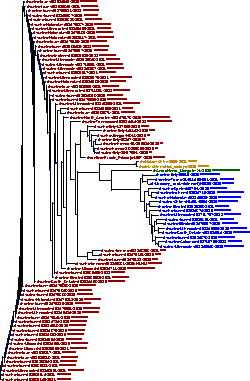
\includegraphics[width=.9\textwidth]{Figures/riskyphylo6_collapsed_19}
% \flushleft

% \fontsize{8}{8}\selectfont
% $^\star$ HA strain is not available for A/duck/New York/1996, so this strain is omitted.\\
% $^{\star\star}$ Could not construct a \qnet of human sequence data available for that virus sub-type (less than 30 strains), so we constructed a \qnet using all human strains that match the HA sub-type, i.e. H5NX for H5N6.\\
% $^{\star\star\star}$ These strains did not have enough human sequence data to generate a \qnet, even when only considering the HA sub-type. Thus, we estimated the risk score using every \qnet from the other IRAT strains, and took the average among NA and HA. Finally, we took the geometric mean of the resulting NA and HA averages.
\captionN{Influenza A Strains Evaluated by IRAT and Corresponding \qnet Computed Risk Scores}\label{highrisktab}
\end{figure}
\else
\refstepcounter{table}\label{highrisktab}
\fi
% #############################################

% \ifFIGS

% \begin{figure}[t]
%   \tikzexternalenable
%   \tikzsetnextfilename{bionorad}
%   \centering
%   \tikzXtrue

  
%   \iftikzX  
%   \begin{tikzpicture}[font=\bf\sffamily\fontsize{8}{8}\selectfont]
  \clip (-2.8in,1.50in) rectangle (3.35in,-0.5in);
\node[anchor=center] (A) at (0,0) {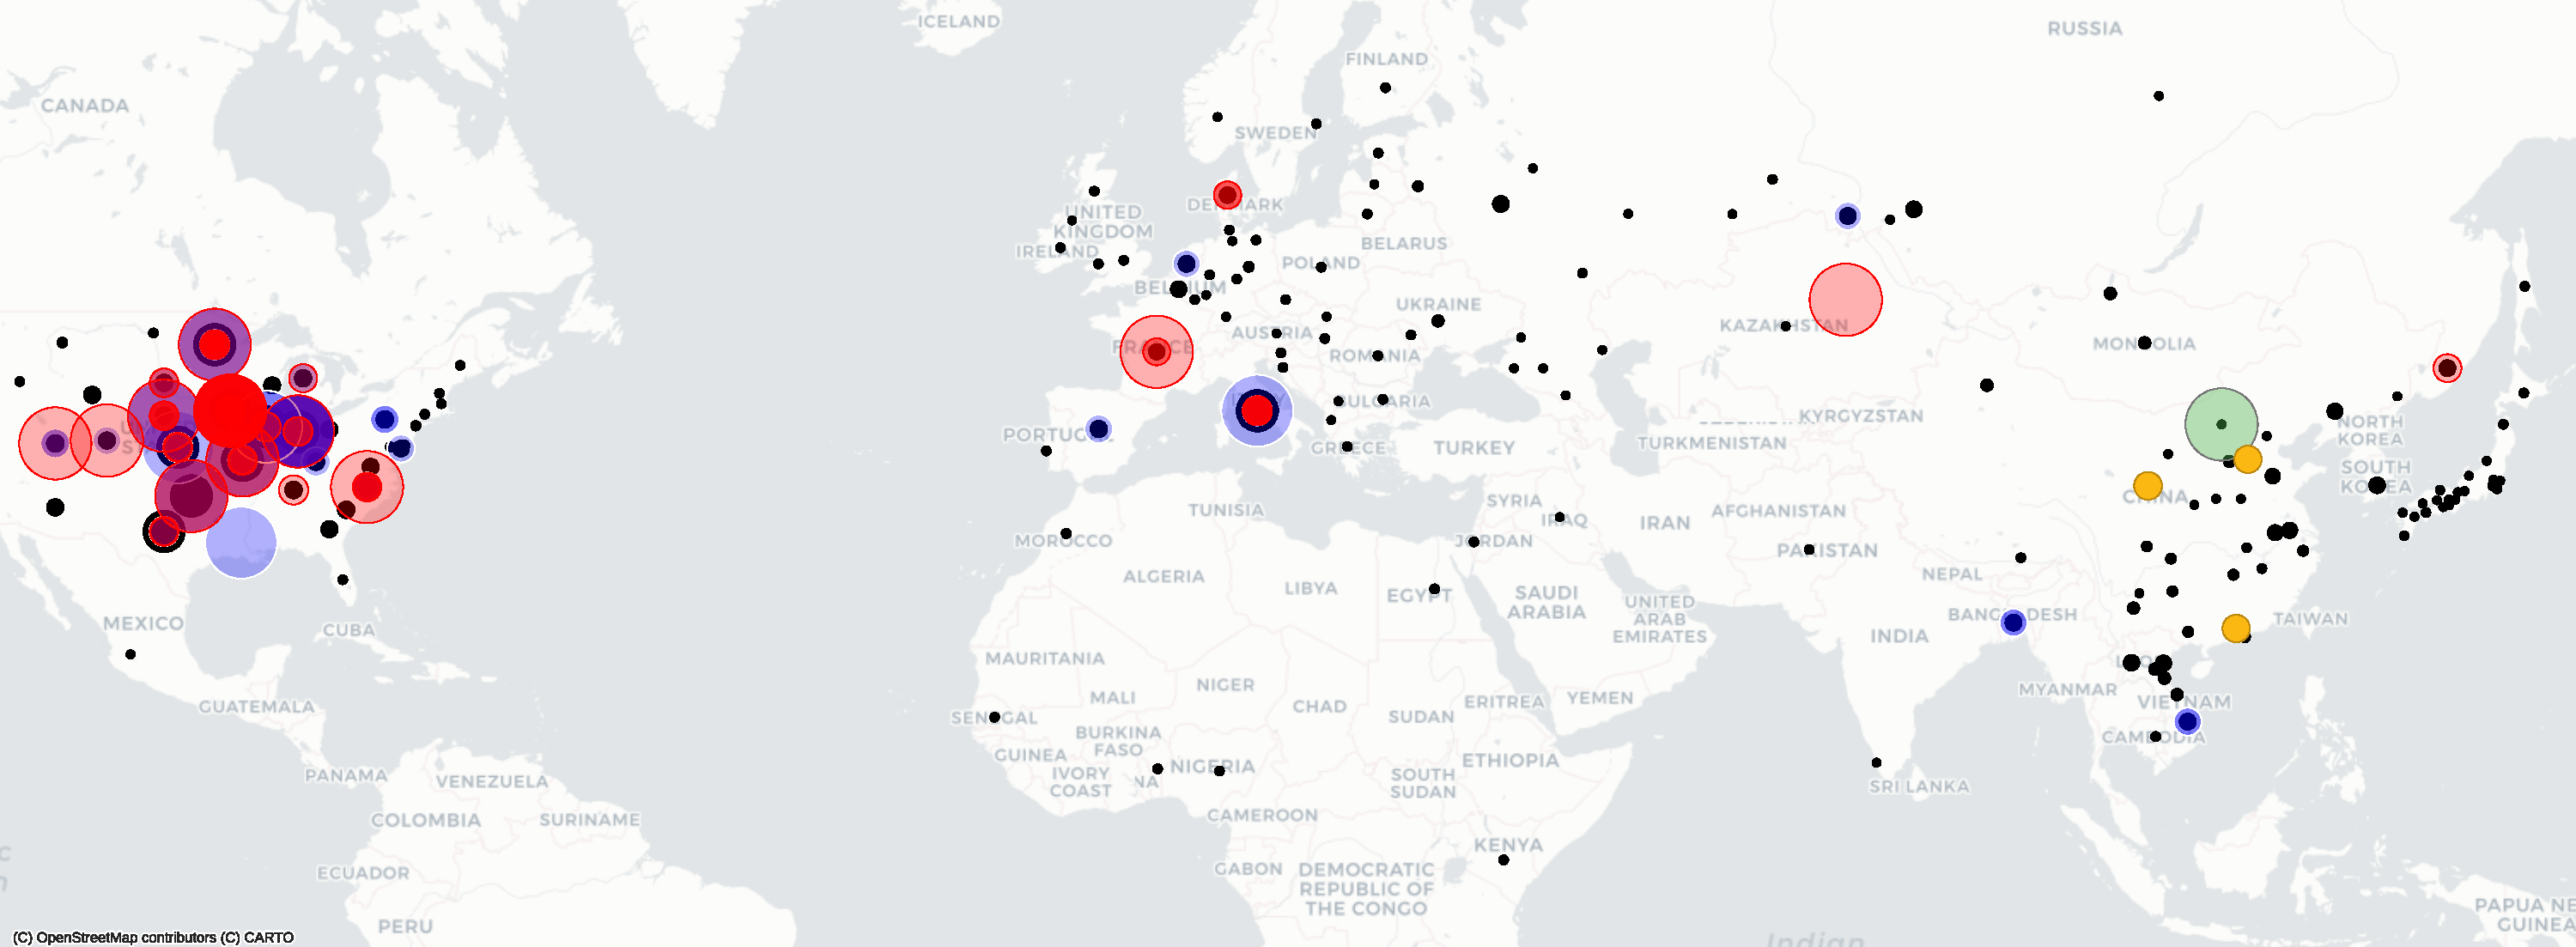
\includegraphics[width=\textwidth]{Figures/bionorad}};
\end{tikzpicture}

%  \else
%   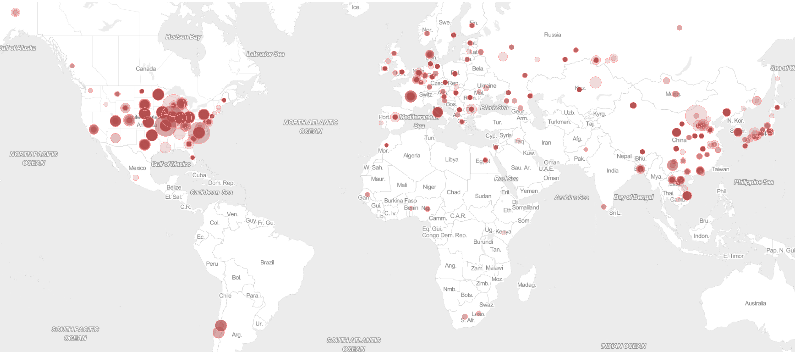
\includegraphics[width=\textwidth]{Figures/External/bionorad}
%   \fi 
%   \vspace{0pt}
% \captionN{Emergence risk evaluation at scale on all 2021-2022 strains collected around the world. 6,254 sequences, total evaluation time: $<$ 15hrs. Size of the markers scale with risk}\label{figbionorad}
% \end{figure}
% \else
% \refstepcounter{figure}\label{figbionorad}
% \fi
